%%%%%%%%%%%%%%%%%%%%%%%%%%%%%%%%%%%%%%%%%%%%%%%%%%%%%%%%%%%%%%%%%%%%%%%%%%%%%%%%
%%%%%%%%%%%%%%%%%%   Vorlage für eine Abschlussarbeit   %%%%%%%%%%%%%%%%%%%%%%%%
%%%%%%%%%%%%%%%%%%%%%%%%%%%%%%%%%%%%%%%%%%%%%%%%%%%%%%%%%%%%%%%%%%%%%%%%%%%%%%%%

% Erstellt von Maximilian Nöthe, <maximilian.noethe@tu-dortmund.de>
% Verändert von Max Pernklau und Matthias Jaeger
% für pdflatex


\documentclass[
  tucolor,
  BCOR=12mm,     % 12mm binding corrections, adjust to fit your binding
  parskip=half,  % new paragraphs start with half line vertical space
  open=any,      % chapters start on both odd and even pages
  cleardoublepage=plain,  % no header/footer on blank pages
]{tudothesis}


% Warning, if another latex run is needed
\usepackage[aux]{rerunfilecheck}

% just list chapters and sections in the toc, not subsections or smaller
\setcounter{tocdepth}{1}

%------------------------------------------------------------------------------
%------------------------------ Sprache und Schrift: --------------------------
%------------------------------------------------------------------------------
\usepackage{lmodern}%Font
\usepackage[T1]{fontenc}
\usepackage[utf8]{inputenc}
\usepackage[parfill]{parskip}%linebreaks instead of indention after paragraphs

% german language
\usepackage[shorthands=off,english,ngerman]{babel}% deutsche Spracheinstellungen

% intelligent quotation marks, language and nesting sensitive
\usepackage[autostyle]{csquotes}

% microtypographical features, makes the text look nicer on the small scale
\usepackage{microtype}
\usepackage{blindtext}

\usepackage[utf8]{inputenc}
%------------------------------------------------------------------------------
%------------------------ Für die Matheumgebung--------------------------------
%------------------------------------------------------------------------------

\usepackage{amsmath}
\usepackage{amssymb}
\usepackage{mathtools}
\usepackage{physics} % bra ket schreibweise mit $\bra{\Psi}\ket{\Psi}$   $\expval{A}{\Psi}$

\usepackage{dsfont}
\usepackage{nicefrac}

\usepackage{adjustbox}

% nice, small fracs for the text with \sfrac{}{}
\usepackage{xfrac}
\usepackage{commath} %propper differentials

%------------------------------------------------------------------------------
%---------------------------- Numbers and Units -------------------------------
%------------------------------------------------------------------------------

\usepackage[
  locale=DE,
  separate-uncertainty=true,
  per-mode=symbol-or-fraction,
]{siunitx}
\sisetup{math-micro=\text{µ},text-micro=µ}

% chemische Formeln
\usepackage[
  version=4,
  math-greek=default, % ┐ mit unicode-math zusammenarbeiten
  text-greek=default, % ┘
]{mhchem}

%------------------------------------------------------------------------------
%-------------------------------- tables  -------------------------------------
%------------------------------------------------------------------------------

\usepackage{booktabs}       % stellt \toprule, \midrule, \bottomrule
\usepackage{grffile}% größere Variation von Dateinamen möglich
\usepackage{pdflscape}% Seite drehen für breite Tabellen

%------------------------------------------------------------------------------
%-------------------------------- graphics -------------------------------------
%------------------------------------------------------------------------------

\usepackage[margin=10pt,font=small,labelfont=bf,labelsep=quad]{caption}
\captionsetup{labelfont={tugreen,bf}}
\usepackage{graphicx}
\usepackage{grffile}

% allow figures to be placed in the running text by default:
\usepackage{scrhack}
\usepackage{float}
\floatplacement{figure}{htbp}
\floatplacement{table}{htbp}

% keep figures and tables in the section
\usepackage[section, below]{placeins}


%------------------------------------------------------------------------------
%---------------------- customize list environments ---------------------------
%------------------------------------------------------------------------------

\usepackage{enumitem}
\usepackage{minted}   % code snippets within text

%------------------------------------------------------------------------------
%------------------------------ Bibliographie ---------------------------------
%------------------------------------------------------------------------------

\usepackage[
  sorting=none,    % sort in order of appearance
  backend=biber,   % use modern biber backend
  autolang=hyphen, % load hyphenation rules for if language of bibentry is not
                   % german, has to be loaded with \setotherlanguages
                   % in the references.bib use langid={en} for english sources
  maxbibnames=99   % no fucking et al.
  %style=numeric,
]{biblatex}
\addbibresource{references.bib}  % die Bibliographie einbinden
\DefineBibliographyStrings{german}{andothers = {{et\,al\adddot}}}
\DeclareFieldFormat{title}{\glqq#1\grqq}
%------------------------------------------------------------------------------
%------------------------------ Sonstiges: ------------------------------------
%------------------------------------------------------------------------------

% Hyperlinks im Dokument
\usepackage[
  unicode,        % Unicode in PDF-Attributen erlauben
  pdfusetitle,    % Titel, Autoren und Datum als PDF-Attribute
  pdfcreator={},  % ┐ PDF-Attribute säubern
  pdfproducer={}, % ┘
  linkbordercolor=tugreen,
  linkcolor=blue, % einfache interne Verkn?pfungen
  citebordercolor=tugreen,
  citecolor=blue, % Verweise auf Literaturverzeichniseintr?ge im Text
]{hyperref}
\usepackage{bookmark}
\usepackage[shortcuts]{extdash}
\usepackage[german]{todonotes}

%------------------------------------------------------------------------------
%------------------------------  Macros:   ------------------------------------
%------------------------------------------------------------------------------

%make parantheses scale in math mode
\makeatletter
\def\resetMathstrut@{%
  \setbox\z@\hbox{%
    \mathchardef\@tempa\mathcode`\[\relax
    \def\@tempb##1"##2##3{\the\textfont"##3\char"}%
    \expandafter\@tempb\meaning\@tempa \relax
  }%
  \ht\Mathstrutbox@\ht\z@ \dp\Mathstrutbox@\dp\z@}
\makeatother
\begingroup
  \catcode`(\active \xdef({\left\string(}
  \catcode`)\active \xdef){\right\string)}
\endgroup
\mathcode`(="8000 \mathcode`)="8000

%increase math spacing between lines with fractions
\makeatletter

\newlength\minalignvsep
\def\align@preamble{%
   &\hfil
    \setboxz@h{\@lign$\m@th\displaystyle{##}$}%
    \ifnum\row@>\@ne
    \ifdim\ht\z@>\ht\strutbox@
    \dimen@\ht\z@
    \advance\dimen@\minalignvsep
    \ht\strutbox\dimen@
    \fi\fi
    \strut@
    \ifmeasuring@\savefieldlength@\fi
    \set@field
    \tabskip\z@skip
   &\setboxz@h{\@lign$\m@th\displaystyle{{}##}$}%
    \ifnum\row@>\@ne
    \ifdim\ht\z@>\ht\strutbox@
    \dimen@\ht\z@
    \advance\dimen@\minalignvsep
    \ht\strutbox@\dimen@
    \fi\fi
    \strut@
    \ifmeasuring@\savefieldlength@\fi
    \set@field
    \hfil
    \tabskip\alignsep@
}
\makeatother

\minalignvsep.15em


\DeclareMathOperator{\const}{const.}

\newcommand{\integral}[4]{\int\displaylimits_{#3}^{#4} #1 \, \mathrm{d} #2}
\makeatletter
\newcommand\primitiveinput[1]
{\@@input #1 }
\makeatother


%------------------------------------------------------------------------------
%------------------------------ New Commands: ---------------------------------
%------------------------------------------------------------------------------
\newcommand{\lvn}{Liouville-von-Neumann Gleichung }
\newcommand*\diff{\mathop{}\!\mathrm{d}}
\newcommand*\Diff[1]{\mathop{}\!\mathrm{d#1}}
\newcommand*\difffrac[2]{\mathop{}\!\frac{\mathrm{d#1}}{\mathrm{d#2}}}
\renewcommand{\pd}[2]{\frac{\mathrm{\partial}#1}{\mathrm{\partial}#2}}
\newcommand{\pdd}[2]{\frac{\mathrm{\partial^2}#1}{\mathrm{\partial}#2^2}}

\newcommand*\inv[1]{#1^{-1}}

\newcommand{\E}[1]{\text{e}^{#1}}
\newcommand{\HR}{\mathcal{H}}

\newcommand*{\estimates}{\stackrel{\scriptscriptstyle\wedge}{=}}

\DeclareSIUnit[number-unit-product = \,]{\permil}{\text{\textperthousand}}

% make text bold instead of italic
% \makeatletter
% \DeclareRobustCommand{\em}{%
%   \@nomath\em \if b\expandafter\@car\f@series\@nil
%   \normalfont \else \bfseries \fi}
% \makeatother

\newcommand*{\english}[1]{\textit{#1}}

% vectors
\newcount\colveccount
\newcommand*\colvec[1]{
        \global\colveccount#1
        \begin{pmatrix}
        \colvecnext
}
\def\colvecnext#1{
        #1
        \global\advance\colveccount-1
        \ifnum\colveccount>0
                \\
                \expandafter\colvecnext
        \else
                \end{pmatrix}
        \fi
}

%------------------------------------------------------------------------------
%------------------------------ RenewCommands: ------------------------------------
%------------------------------------------------------------------------------
\DeclareMathOperator{\spn}{span}
\renewcommand{\vec}[1]{\mathbf{#1}}

%------------------------------------------------------------------------------
%-------------------------    Angaben zur Arbeit   ----------------------------
%------------------------------------------------------------------------------

\author{Matthias Jaeger}
\title{Diskontinuierliche Galerkin Methoden zur Lösung der Liouville-von-Neumann-Gleichung}
\date{\today}
\birthplace{Würselen}
\chair{Lehrstuhl für Hochfrequenztechnik}
\division{Fakultät Physik}
\thesisclass{Master of Science}
\publishers{\thechair \\ \thedivision \\ Technische Universität Dortmund}
\submissiondate{17. Juli 2019}
\firstcorrector{Prof.~Dr.~Manfred Bayer}
\secondcorrector{PD.~Dr.~Dirk Schulz}

% tu logo on top of the titlepage
\titlehead{\includegraphics[height=1.5cm]{logos/tu-logo.pdf}}

\begin{document}
\frontmatter
\maketitle

% Gutachterseite
\makecorrectorpage

\chapter{Einleitung}
Quantenstrukturen, wie sie heutzutage hergestellt werden können, eröffnen neue Möglichkeiten im Bereich der ultraschnellen Elektronik und Photonik. Solche Strukturen lassen sich in aller Regel als \emph{offene} Systeme beschreiben. Es findet ein Austausch von lokal erhaltenen Fermionen -- die Erhaltung wird durch eine lokale Kontinuitätsgleichung beschrieben -- mit der Umgebung statt. Die Umgebung besteht dabei aus mindestens zwei verschiedenen Teilchen-Reservoirs. In diesem Fall kann also ein Nicht-Gleichgewichtszustand erreicht werden, beispielsweise durch das Anlegen einer Spannung. Das zu untersuchende System besitzt eine endliche Ausdehnung im Raum. Es muss im Nicht-Gleichgewichtsfall folglich ein Strom durch die Oberfläche als Rand des Systems fließen. Wir beschränken uns hier auf eindimensionale Quantenstrukturen, für die also die interessante Physik in einer Dimension stattfindet. Dabei wollen wir den Strom der Teilchen, also den quantenmechanischen Transport beschreiben. Dies geschieht allgemein in verschiedenen Anwendungsfällen (Hydrodynamik, Aerodynamik, Elektronik, Neutronentransport, \dots) mit Hilfe einer die Dynamik beschreibenden Differentialgleichung. Hierfür werden Randbedingungen benötigt. Eben diese Randbedingungen definieren den offenen (oder auch geschlossenen) Charakter des Systems.

\chapter{Problemstellung}

\section{Dichteoperator und Dichtematrix}
Aus Ingenieurs-Sicht ist es sehr natürlich, nach der Elektronendichte $n(\vb{r})$ in einem System zu fragen. Quantenmechanisch ist diese Größe eine Observable, also der Erwartungswert eines hermitschen Operators bezüglich des Hilbertraums der $L^2$-Funktionen. Anschaulich ist klar, dass sich die Elektronendichte aus zwei Wahrscheinlichkeiten zusammensetzt. Erstens benötigen wir die Wahrscheinlichkeit dafür, dass ein Zustand mit Energie $\epsilon$ besetzt ist. Diese wird mit der  Aufenthaltswahrscheinlichkeit, dass am Ort $\vb{x}$ überhaupt ein Teilchen vorhanden ist, multipliziert. Im Gleichgewicht ergibt sich mit $\epsilon_{\alpha}$ als Eigenwerte und $\Psi_{\alpha}$ als Eigenvektoren des Hamiltonoperators \cite{datta}
\begin{align}
  n(\vb{r}) = \sum_{\alpha} \sum_{\beta} C_{\alpha} C_{\beta}^*\Psi_{\alpha}(\vb{r}) \Psi_{\beta}^*(\vb{r})
\end{align}
mit $|C_{\alpha}|^2 = f(\epsilon_{\alpha}-\mu)$, der mittleren Besetzungszahl für wechselwirkungsfreie Teilchen, gegeben durch
\begin{align}
  f(E) = \frac{1}{1+\exp(\beta E)} \; .
\end{align}
Wir bezeichnen mit $\tilde{\rho}(\alpha,\beta) = f_a\delta_{a,\beta}$ den diagonalen Dichteoperator in der Energie-Darstellung und schreiben allgemein
\begin{align}
  \rho(\vb{r},\vb{r}') \equiv \sum_{\alpha} \sum_{\beta} \tilde{\rho}(\alpha,\beta)\Psi_{\alpha}(\vb{r})\Psi^*_{\beta}(\vb{r}') \; ,
  \label{eq:unitTrafo}
\end{align}
sodass die Elektronendichte sich aus der Dichtematrix in Ortsdarstellung aus
\begin{align}
  n(\vb{r}) = \rho(\vb{r},\vb{r})
\end{align}
ergibt.
Wir konzentrieren uns im folgenden lediglich auf ein Modell unabhängiger Elektronen in einer Dimension, sodass es genügt, die Einteilchen-Dichtematrix zu betrachten.

Die Gleichung \eqref{eq:unitTrafo} stellt eine unitäre Transformation $\rho = V\tilde{\rho}V^{\dagger}$ mit $[V]_{\vb{r},\alpha} = \Psi_{\alpha}(\vb{r})$ dar. Unter Kenntnis der Eigenvektoren und -werte des Hamiltonoperators könnten wir also direkt die Dichtematrix in Ortsdarstellung erhalten. Dies gilt jedoch lediglich im Gleichgewichts-Fall.

Für zeitabhängige Probleme betrachten wir stattdessen direkt die Bewegungsgleichung für den Dichteoperator $\hat{\rho}$ -- die von-Neumann-Gleichung -- und daraus abgeleitet die Bewegungsgleichung für die Dichtematrix im Ortsraum $\rho(x,x')$ -- die \lvn. Der Zusammenhang zwischen Operator und Matrix ist gegeben durch
\begin{align}
  \rho(x,x') &= \bra{x} \hat{\rho} \ket{x'} \\
  &= \bra{x} (\sum_{\alpha} p_{\alpha} \ket{\Psi_{\alpha}}\bra{\Psi_{\alpha}}) \ket{x'} \; ,
\end{align}
wobei $p_{\alpha}$ die Eigenwerte von $\hat{\rho}$ sind.

\section{Herleitung der Liouville-von-Neumann Gleichung}
Die Liouville-von-Neumann Gleichung erhalten wir aus der von-Neumann-Gleichung wie folgt.
\begin{align}
  \td{\hat{\rho}}{t} &= \frac{i}{\hbar}\left[\hat{\rho} , H\right] \\
  \underbrace{\bra{x} \td{\hat{\rho}}{t} \ket{y}}_{= \partial_t \rho(x,y,t)} &= \bra{x}\ket{\frac{i}{\hbar}\left[\hat{\rho} , H\right]y} \\
   &= \frac{i}{\hbar} \sum_{\alpha} p_{\alpha} ( \underbrace{\bra{x}\ket{\Psi_{\alpha}}}_{\equiv \Psi_{\alpha}(x)}\bra{\Psi_{\alpha}}\ket{Hy} - \bra{x}\ket{H\Psi_{\alpha}}\underbrace{\bra{\Psi_{\alpha}}\ket{y}}_{\equiv \Psi_{\alpha}^*(y)} )
\end{align}
Mit dem Hamiltonoperator für ein einzelnes Teilchen in einer Dimension in Ortsdarstellung
\begin{align}
  \left[ -\frac{\hbar^2}{2m}\frac{\partial^2}{\partial x^2} + V(x,t) \right] \Psi(x,t) = \bra{x}\ket{H\Psi} \equiv \mathcal{L}(x,t)\Psi(x,t)
  \label{eq:Liouville-Operator}
\end{align}
folgt mit $H^{\dagger} = H$ und temporärer Unterdrückung der Zeitabhängigkeit
\begin{align}
  \partial_t \rho(x,y,t) &= \frac{i}{\hbar} \sum_{\alpha} p_{\alpha} \left( \Psi_{\alpha}(x)\mathcal{L}^*(y)\Psi_{\alpha}^*(y) - \mathcal{L}(x)\Psi_{\alpha}(x)\Psi_{\alpha}^*(y) \right) \\
  &= \frac{i}{\hbar}  (\mathcal{L}^*(y) - \mathcal{L}(x)) \sum_{\alpha} p_{\alpha} \left( \Psi(x)\Psi^*(y) \right) \\
  &= \frac{i}{\hbar}  (\mathcal{L}^*(y) - \mathcal{L}(x)) \bra{x}\left(\sum_{\alpha} p_{\alpha}  \ket{\Psi_{\alpha}}\bra{\Psi_{\alpha}} \right)\ket{y} \\
  &= \frac{i}{\hbar}  (\mathcal{L}^*(y) - \mathcal{L}(x))\rho(x,y)
\end{align}
Wir definieren noch
\begin{align}
  \mathcal{L}(x,y) &\equiv \mathcal{L}(x) - \mathcal{L}^*(y)\\
   &= -\frac{\hbar^2}{2m}\left( \partial_x^2 - \partial_y^2 \right) + V(x) - V^*(y)
\end{align}
und erhalten die Liouville-von-Neumann Gleichung im Ortsraum
\begin{equation}
  \partial_t \rho(x,y,t) = \frac{1}{i\hbar} \mathcal{L}(x,y,t) \rho(x,y,t) \; .
  \label{eq:lvn_first}
\end{equation}
Es lassen sich zwei Fälle unterscheiden:
\begin{itemize}
  \item Der stationäre Fall mit $\partial_t \rho(x,y,t) = 0$
  \item der allgemeinere transiente Fall $\partial_t \rho(x,y,t) \neq 0$.
\end{itemize}

\section{Schwerpunkt- und Relativkoordinaten}
Wir führen die Schwerpunkt- und Relativkoordinaten
\begin{align}
  &r \equiv \frac{x+y}{2} \qquad &q \equiv x-y \label{eq:gedrehteKoordinaten}\\
  \Leftrightarrow\qquad &x = r+\frac{q}{2} \qquad &y = r-\frac{q}{2}
\end{align}
ein. Die Ableitungen transformieren sich dabei gemäß
\begin{align}
  \partial_r \partial_q  &= \partial_r \left( \frac{\partial}{\partial x} \frac{\partial x}{\partial q} + \frac{\partial}{\partial y} \frac{\partial y}{\partial q}\right) \\
   &= \left( \frac{\partial}{\partial x} \frac{\partial x}{\partial r} + \frac{\partial}{\partial y} \frac{\partial y}{\partial r}\right) \left( \frac{\partial}{\partial x} \frac{1}{2} + \frac{\partial}{\partial y} \frac{-1}{2}\right)\\
    &= \left( \frac{\partial}{\partial x} 1 + \frac{\partial}{\partial y} 1\right) \left( \frac{\partial}{\partial x} \frac{1}{2} + \frac{\partial}{\partial y} \frac{-1}{2}\right)\\
   &= \frac{1}{2}\partial_x \partial_x - \frac{1}{2}\partial_x \partial_y + \frac{1}{2}\partial_y \partial_x - \frac{1}{2}\partial_y \partial_y \\
  &=  \frac{1}{2}(\partial_x^2 - \partial_y^2) \; ,
\end{align}
wobei im letzten Schritt der Satz von Schwarz genutzt wird. Damit ergibt sich der transformierte Liouville Operator zu
\begin{align}
  \mathcal{L}(r,q,t) = -\frac{\hbar^2}{m} \partial_r\partial_q + \underbrace{V\left(r+\frac{q}{2},t\right) - V^*\left(r-\frac{q}{2},t\right)}_{\equiv \tilde{B}(r,q,t)} \; .
\end{align}
Mit der Umbenennung
\begin{align*}
  \rho \longrightarrow u \\
  r \longrightarrow \tilde{x} \\
  q \longrightarrow \tilde{y} \\
  t \longrightarrow \tilde{t}
\end{align*}
sowie der Definition
\begin{align}
  A = \left(\begin{array}{c c} 0 & \frac{1}{2} \\ \frac{1}{2} & 0 \end{array} \right)
\end{align}
lautet die LvN Gleichung nun
\begin{align}
  i\hbar\partial_{\tilde{t}} u(\tilde{x},\tilde{y},\tilde{t})+\frac{\hbar^2}{m}\operatorname{div}(A\nabla u(\tilde{x},\tilde{y},\tilde{t})) -  \tilde{B}(\tilde{x},\tilde{y},\tilde{t}) u(\tilde{x},\tilde{y},\tilde{t}) = 0
\end{align}

\section{Charakteristische Einheiten}
Zunächst wird die  \lvn in eine einheitenlose Form gebracht.
\begin{align}
    i\frac{\hbar}{V_0}\partial_{\tilde{t}}\, u(\tilde{x},\tilde{y},\tilde{t})+\frac{\hbar^2}{mV_0}\operatorname{div}(A\nabla u(\tilde{x},\tilde{y},\tilde{t})) - \frac{\tilde{B}(\tilde{x},\tilde{y},\tilde{t})}{V_0} u(\tilde{x},\tilde{y},\tilde{t}) = 0
\end{align}
Energien werden in Einheiten von $V_0$ gemessen, welche wir im weiteren Verlauf als die Potentialbarriere $V_0 = \SI{0.1768}{\electronvolt}$ wählen werden.

Wir führen folgende Skalierung ein, um nun auch Zeiten und Orte einheitenlos zu behandeln.
\begin{align}
  \left(\begin{array}{c}\tilde{x}\\\tilde{y}\end{array}\right) &= \xi \left(\begin{array}{c}x\\y\end{array}\right)   & \xi &= \sqrt{\frac{\hbar^2}{mV_0}} \\
  \tilde{t} &= \tau t   & \tau &= \frac{\hbar}{V_0}
\end{align}
Damit folgt
\begin{align}
  \partial_{\tilde{t}} &= \frac{\partial}{\partial (\tau t)} = \tau^{-1} \partial_t = \frac{V_0}{\hbar} \partial_t \\
  \partial_{\tilde{x}}^2 &= \frac{\partial^2}{(\partial (\xi x))^2} = \xi^{-2} \partial_x^2 = \frac{mV_0}{\hbar^2} \partial_x² \; ,
\end{align}
sodass die \lvn die Form
\begin{empheq}[box=\widefbox]{align}
  i \partial_t u(x,y,t)+\operatorname{div}(A\nabla u(x,y,t)) - B(x,y,t) u(x,y,t) = 0
  \label{eq:lvn}
\end{empheq}
annimmt. Hierbei ist
\begin{align}
  B(x,y,t) \equiv \frac{\tilde{B}(x,y,t)}{V_0} = \frac{V\left(x+\frac{y}{2},t\right) - V^*\left(x-\frac{y}{2},t\right)}{V_0}
\end{align}
eingeführt worden. Die Skalierung lässt sich berechnen, indem die effektive Masse als konstant
\begin{align}
  m = 0.063 m_0 =  0.063\cdot\SI{9.1e-31}{\kilogram}
\end{align}
angenommen wird. Damit ergibt sich folgende Skalierung zwischen SI-Einheiten und den hier eingeführten einheitenlosen Größen.
\begin{align}
  V_0 &= \SI{0.1768}{\electronvolt} \\
  \xi &= \SI{6.57e-10}{\meter}
 \\
  \tau &= \SI{3.72e-15}{\second}

\end{align}

\section{Mathematische Aspekte der \lvn}
Die eindimensionale Wellenfunktion $\Psi(x)$ eines Teilchens ist ein Vektor des unendlich-dimensionalen Hilbertraums $L^2(\mathbb{R})$ mit dem üblichen Skalarprodukt
\begin{align}
  \bra{\Psi}\ket{\Phi} = \int_{\mathbb{R}} \Psi^*(x)\Phi(x) \diff x \; .
\end{align}
Beschränken wir uns auf ein Rechengebiet $L$, so ist entsprechend $\Psi(x) \,\in\,L^2(L)$. Diskretisieren wir ferner das System, so wird der Hilbertraum endlichdimensional mit Dimension $N$. Dann ist die Dichtematrix in Gleichung \eqref{eq:lvn} eine Matrix der Form $\mathbb{C}^N \times \mathbb{C}^N$ und der Liouville-Operator ein "Superoperator" \cite{frensley2} der Form $(\mathbb{C}^N \times \mathbb{C}^N)\times(\mathbb{C}^N \times \mathbb{C}^N)$. Letztlich wird numerisch gesehen $N^2$ der Anzahl Freiheitsgrade entsprechen und die \lvn wird wieder eine Matrix-Vektor-Gleichung sein. Dazu wird $u(x,y)$ nicht als Matrix, sondern als Vektor der Länge $N^2$ geschrieben.
\todo{Eigenschaften von B(x,y) und A. Hermitizität von $\mathcal{L}$ (frensley).}

\section{Randbedingungen}
Die Dynamik des in der Einleitung skizzierten Systems muss irreversibel in der Zeit sein. Andernfalls sind instabile Lösungen in der Zeit zulässig \cite{frensley2}. Solche instabilen Lösungen lassen sich anhand des Eigenwertspektrums des Liouvilleoperators aus Gleichung \eqref{eq:lvn_first} erkennen. Es lässt sich zeigen, dass für geschlossene, konservative Systeme $\mathcal{L}$ hermitsch ist als Folge der Hermitizität des Hamiltonoperators $H$ \cite{frensley2}.
\begin{align}
  H- H^{\dagger} = \frac{\hbar}{i}\int_s \vb{j}\diff\vb{s} = 0
\end{align}
Der Nettostrom durch die Oberfläche ist also Null. Damit treten lediglich oszillierende Lösungen der \lvn auf. Da wir nun offene Systeme modellieren wollen, müssen wir das Ein- und Austreten von Teilchen in das System erlauben und verletzen dadurch die Hermitizität von $H$ und $\mathcal{L}$. Dadurch wird mindestens ein Eigenwert einen nicht-verschwindenden imaginären Teil bekommen. Anhand Gleichung \eqref{eq:lvn_first} sehen wir, dass in der Zeit instabile Lösungen für Eigenwerte mit positivem Realteil auftreten. Falls die Randbedingungen reversibel in der Zeit sind, so sind die Realteile der Eigenwerte symmetrisch und es existieren unphysikalische, instabile Lösungen \cite{frensley2}. Ein Beispiel hierfür ist $\partial \rho /\partial r = 0$ entlang $x=0$ und $y=0$. Diese Randbedingung ist insofern plausibel, da sie zu konstanter Dichte an den Rändern führt und damit den Effekt eines fixierten chemischen Potentials beschreibt. Sie führt jedoch wegen der Zeit-Umkehrbarkeit zu unphysikalisch exponentiell steigenden Lösungen.

Die Randbedingungen müssen also irreversibel in der Zeit sein und ferner die Stabilität des Systems sicherstellen. Ein hierfür geeigneter Ansatz wird erstmals in \cite{frensley2} getroffen, indem die Reservoire in Analogie zu einem schwarzen Körper gesehen werden. In das Reservoir eintretende Teilchen werden vollständig absorbiert. Umgekehrt "strahlt" das Reservoir Teilchen entsprechend der thermischen Gleichgewichts-Verteilung in das System ein. Damit ist klar, dass Randbedingungen für \emph{Inflow-}Teilchen mit positiver Geschwindigkeit am linken Rand und solche mit negativer Geschwindigkeit am rechten Rand gesetzt sind, während für \emph{Outflow}-Teilchen keine Randbedingung vorgegeben ist. Wir müssen also dazu in der Lage sein, Teilchen nach ihrer Geschwindigkeit zu unterscheiden.
Es ist daher ein natürliches Vorgehen, nach einer Wahrscheinlichkeitsverteilung im Phasenraum zu fragen. Dieser Frage ging Eugene Wigner 1932 nach \cite{wigner} und formulierte die nach ihm benannte Wignerverteilung $P(r, k)$, siehe Kapitel \ref{sec:wignerfunktion}. Die klassische Position eines Teilchens wird dann mit $r$ aus Gleichung \eqref{eq:gedrehteKoordinaten} und der klassische Impuls mit $p=\hbar k$ identifiziert.
Dabei ist $k$ die zu $q$ aus Gleichung \eqref{eq:gedrehteKoordinaten} gehörende Wellenzahl. Positive und negative Geschwindigkeiten lassen sich einfach durch das Vorzeichen von $k$ unterscheiden, sodass sich die Randbedingungen konkretisieren lassen.
\begin{align}
  P(-L/2,k)|_{k>0} &= f_l(k) \\
  P(+L/2,k)|_{k<0} &= f_r(k)
\end{align}
Die Gleichgewichts-Verteilung der Reservoire $f_{l,r}(k)$ ergibt sich aus der Fermi-Dirac-Statistik wie folgt durch Integration über die zwei senkrecht zu $k\equiv k_z$ stehenden Wellenzahlen.
\begin{align}
  \frac{\expval{N}}{A_{\perp}} &= 2\frac{1}{A_{\perp}}\sum_{\vb{k}}\frac{1}{1+\exp(\beta(\epsilon(\vb{k}) - \mu))} \\
    &= 2\frac{1}{A_{\perp}}  \frac{A_{\perp}}{(2\pi)^2} \sum_{k_z}\int_{-\infty}^{\infty} \diff k_y \int_{-\infty}^{\infty} \diff k_x \frac{1}{1+\exp(\beta(k_x^2 + k_y^2 + k_z^2)\frac{\hbar^2}{2m} - \mu)} \\
    &= \frac{2}{(2\pi)^2} \sum_{k_z} \int_0^{2\pi} \diff \varphi \int_0^{\infty} \diff k_{\perp} k_{\perp} \frac{1}{1+\exp(\beta(k_{\perp}^2 + k_z^2)\frac{\hbar^2}{2m} - \beta \mu)}
\end{align}
Wir substituieren $\epsilon = (k^2_{\perp} + k_z^2)\frac{\hbar^2}{2m} - \mu$ und somit $\diff k_\perp = \frac{m}{\hbar^2 k}\diff \epsilon$. Für das Integral nutzen wir $\td{}{x}\ln(1+\exp(-\beta x)) = -\beta / (1+\exp(\beta x))$ und folgern weiter
\begin{align}
  \frac{\expval{N}}{A_{\perp}} &= \frac{4\pi}{(2\pi)^2} \frac{m}{\hbar^2} \sum_{k_z} \int_{\epsilon(0)}^{{\epsilon(\infty)}} \diff \epsilon \frac{1}{1+\exp(\beta\epsilon)} \\
    &= \frac{m}{\pi\hbar^2}\left( \frac{-1}{\beta}\right) \sum_{k_z} \left.\ln(1+\exp(\beta(k_{\perp}^2 + k_z^2)\frac{\hbar^2}{2m} + \beta\mu))\right|_0^{\infty} \\
    &= \sum_{k_z} \frac{m}{\pi\hbar^2\beta} \ln(1+\exp(\beta(\frac{- k_z^2\hbar^2}{2m} + \mu)))
\end{align}
Für lokal konstantes $\beta$ erhalten wir daher in Übereinstimmung mit \cite{frensley2} die Randbedingungen
\begin{align}
  f_{l,r} (k) = \frac{m}{\pi\hbar^2\beta} \ln(1+\exp(\beta(\frac{- k^2\hbar^2}{2m} + \mu_{l,r}))) \; .
\end{align}
\todo{Wie bauen wir das in die \lvn in Ortsdarstellung ein, ohne zum Wigner-Formalismus überzugehen?}


\section{Strom- und Ladungsträgerdichte}
Aus der Dichtematrix $\rho(r,q,t)$ in Schwerpunkt- und Relativkoordinaten lassen sich Strom- und Ladungsträgerdichte ableiten. Es gilt \cite{lukas1}
\begin{align}
  j(r,t) &= \frac{\hbar}{m}\Im{\partial_q \rho(r,q,t)|_{q=0}} \\
  n(r,t) &= \Re{\rho(r,q,t)|_{q=0}} \; .
  \label{eq:dichte}
\end{align}

\section{Selbstkonsistentes Potential}
Das Potential in dem Liouville-Operator \eqref{eq:Liouville-Operator} setzt sich zusammen aus dem Hartree Potential $u(x,y,z)$, dem Heterostuktur Potential $V_s(x,y,z)$ sowie dem äußeren Feld $-eU$.
\begin{align}
  V(\vb{x}) = u(\vb{x}) + V_s(\vb{x}) - eU
\end{align}
Auch hier lassen sich wieder zwei Fälle unterscheiden.
\begin{itemize}
  \item Der Gleichgewichtsfall $U=0$. %Hier kann als Randbedingung auf beiden Seiten die Fermi-Dirac-Statistik \eqref{eq:fd_statistic} angenommen werden.
  \item Der Nicht-Gleichgewichtsfall $U\neq 0$. %Hier sind lediglich die \emph{inflow}-Bedingungen für positive Geschwindigkeiten am linken- und negative Geschwindigkeiten am rechten Rand des Rechengebietes bekannt.
\end{itemize}
Da das Hartree Potential von der Konstellation der Elektronen abhängt und umgekehrt, wird es selbstkonsistent berechnet, wie im folgenden Abschnitt erläutert wird.

\subsection{Hartree-Potential}
Das Hartree Potential ist mit der Elektronendichte $n(\vb{x})$ durch die Poisson-Gleichung \cite{frensley}
\begin{align}
  -\div \epsilon(\vb{x}) \grad u(\vb{x}) = e^2 (n(\vb{x}) - N_D(\vb{x})) \; ,
  \label{eq:poisson_3d}
\end{align}
verknüpft, wobei $N_D(\vb{x})$ die ortsabhängige Dichte der Donatoren in der Heterostuktur und $\epsilon(\vb{x})$ die Permittivität bezeichnet. Akzeptoren und Löcher werden aufgrund der Dotierung $N_D \gg N_A$ vernachlässigt. Ferner nehmen wir aufgrund der eindimensionalen Problemstellung an, dass $u(\vb{x}) = u(x)$ und $\epsilon(\vb{x})=\epsilon(x)$ sodass die Poisson-Gleichung eindimensional wird.
\begin{align}
  -\partial_x (\epsilon(x)\partial_x u(x)) = e^2(n(x)-N_D(x))
  \label{eq:poisson}
\end{align}
Die Randbedingungen für $u$ ergeben sich aus der Forderung nach Ladungsneutralität in ausreichend großer Entfernung  \cite{frensley}
\begin{align}
  u|_{\partial\Omega} = \mu(\vb{x})|_{\partial\Omega}-V_s(\vb{x})|_{\partial\Omega}-\frac{1}{\beta}\mathcal{F}_{1/2}^{-1}(N_D/N_C) \; .
  \label{eq:RB_PE}
\end{align}
Hierin ist $\mu(\vb{x})$ das chemische Potential, $\beta=1/(k_BT)$ mit $T=\SI{300}{\kelvin}$, $N_C = 2(m^*/2\pi\hbar^2\beta)^{3/2}$ die "effektive Zustandsdichte" und $\mathcal{F}_{1/2}$ das Fermi-Dirac Integral der Ordnung $1/2$:
\begin{align}
  \mathcal{F}_j(x)=\frac{1}{\Gamma(j+1)}\int_0^{\infty}\frac{t^j}{\exp(t-x)+1}\diff t
\end{align}
Das Potential ergibt sich nach Gleichungen \eqref{eq:poisson} und \eqref{eq:dichte} aus dem Dichteoperator -- umgekehrt ergibt sich der Dichteoperator nach Gleichung \eqref{eq:lvn} aus dem Potential. Die Beziehung zwischen Potential und Dichte ist nicht-linear. Die gleichzeitige Lösung für Poisson- und \lvn zu finden erfordert daher Iteration. Das Problem wird \emph{selbstkonsistent} gelöst. Dazu wird $\eqref{eq:lvn}$ zunächst mit einem geeigneten \emph{initial guess} $V^{(0)}$ gelöst. Nun wird iteriert und alternierend gelöst, bis Dichte und Potential sich nicht mehr signifikant ändern. Im Fall der transienten Betrachtung entspricht eine Iteration gleichzeitig einem Zeitschritt. Das Verfahren ist als \emph{Gummel (Plug-in) Approach} etabliert und beispielsweise in \cite{gummel} beschrieben. Die folgenden Ausführungen orientieren sich an dieser Literaturquelle.

Numerisch behandeln wir Gleichung \eqref{eq:poisson} mit dem Finite-Differenzen Verfahren. Das Rechengebiet $L$ wird diskretisiert gemäß
\begin{align}
  L_N \equiv \{x_i | x_i = i h \,\forall\, i = 0,1,\dots,N\text{ mit }L=Nh\}
\end{align}
Aus der Taylorentwicklung einer Funktion $f:L \rightarrow \mathbb{R}$ folgt für die Ableitungen
\begin{align}
  f'(x_i) &= \frac{f(x_{i+1}) - f(x_{i-1})}{2h} + \mathcal{O}(h^2) \\
  f''(x_i) &= \frac{f(x_{i+1}) - 2f(x_i) + f(x_{i-1})}{h^2} + \mathcal{O}(h^2) \; .
\end{align}
Wir schreiben kurz $f(x_i)\equiv f_i$.
Damit lässt sich mit $a_i\equiv (\epsilon_{i+1} - \epsilon_{i-1})/(4h^2\epsilon_i)$ Gleichung \eqref{eq:poisson} umschreiben zu
\begin{align}
  u_{i+1}\cdot(1+a_i) -2 u_i + u_{i-1}\cdot(1-a_i) - \underbrace{e^2h^2\frac{(N_{D,i} - n_i)}{\epsilon_i}}_{\equiv \text{rhs}_i} = 0\; ,
  \label{eq:discretePE}
\end{align}
wobei berücksichtigt werden muss, dass $u_0$ und $u_N$ über die Randbedingungen nach Gleichung \eqref{eq:RB_PE} vorgegeben sind. Somit haben wir das LGS
\begin{align}
  \left[ \begin{matrix}-2 & 1+a_1 & & & 0\\1-a_2 & \ddots & \ddots & & \\ & \ddots & \ddots & \ddots & \\& & \ddots & \ddots &  1+a_{N-2} \\0 & &  & 1-a_{N-1} & -2  \end{matrix}  \right]
  \left[ \begin{matrix}u_1             \\                          \\ \vdots                       \\                           \\u_{N-1}  \end{matrix}  \right]
  = \left[ \begin{matrix}\text{rhs}_1  \\                          \\ \vdots                       \\                         \\\text{rhs}_{N-1}  \end{matrix}  \right]
   - \left[ \begin{matrix}(1-a_1)u_0     \\0                         \\ \vdots                      \\0                        \\(1+a_{N-1})u_N  \end{matrix}  \right]
\end{align}
zu lösen. An dieser Stelle halten wir kurz inne und fragen uns, ob wir nicht eine "bessere" Vorhersage für $u^{(n+1)}$ treffen können, sodass wir eine schnellere Konvergenz der Iteration erreichen können. Diese Überlegung führt uns auf das verallgemeinerte Newton-Raphson-Verfahren.
Die linke Seite von Gleichung \eqref{eq:discretePE} definieren wir als Funktion $P_i(u_1,\dots,u_N)$ und wenden hierauf das Newton-Raphson-Verfahren an. Ausgehend von einem Startwert $\vb{u}^{(0)}$ erhalten wir das Fixpunktproblem
\begin{align}
  \vb{u}^{(n+1)} = \vb{u}^{(n)} - (\mathrm{D}\vb{P}|_{\vb{u}^{(n)}})^{-1} \vb{P}(\vb{u}^{(n)}) \; ,
  \label{eq:fixpunkt_gummel}
\end{align}
wobei wir die Vektorschreibweise
\begin{align}
  \vb{f} = \left( f_0,\dots,f_N\right)^T = \left( f(x_0),\dots,f(x_N)\right)^T
\end{align}
eingeführt haben und $\mathrm{D}$ der Differentiationsoperator ist, in diesem Fall also die Jacobik Matrix von $P$.
\begin{align}
  \left(\mathrm{D}\vb{P}|_{\vb{u}^{(n)}}\right)_{i,j} &= \pd{P_i}{u_j^{(n)}} \\ &\stackrel{\eqref{eq:discretePE}}{=}
  (1+a_i)\delta_{i+1,j} - 2 \delta_{i,j} + (1-a_i)\delta_{i-1,j} + \frac{e^2h^2}{\epsilon_i}\pd{n_i^{(n)}}{u_j^{(n)}}
\end{align}
An dieser Stelle ist anzumerken, dass nun auch die Dichte $n$ einen Iterationsindex $(n)$ bekommen hat. Dies ist auf die eingangs beschriebene alternierende Iteration zurückzuführen, in welcher abwechselnd $n^{(n)}$ und $u^{(n)}$ in einem einzigen Iterationsschritt $(n)$ berechnet werden. Ferner ist die Ableitung $\pd{n_i^{(n)}}{u_j^{(n)}}$ zunächst nicht bekannt.
Es ist überhaupt eine Abweichung $\pd{n_i^{(n)}}{u_j^{(n)}} \neq 0$, die den Unterschied zwischen Newton-Iteration und direktem Lösen bewirkt. Im Allgemeinen liegt keine exakte Form dieser Ableitung vor, da hierzu ja gerade die \lvn zu lösen ist. Es lässt sich jedoch eine Abschätzung vornehmen, welche schnell und kostengünstig ist, sodass das Newton-Verfahren einen echten Vorteil gegenüber dem direkten Iterieren hat. Dazu bedienen wir uns der Maxwell-Boltzmann-Statistik
\begin{align}
  n(u) = N_0\exp\left(\frac{u-u_0}{k_B T}\right)
  \label{eq:maxwell_boltzmann}
\end{align}
als klassisches Gleichgewichts-Resultat. Dies ist wohlgemerkt eine Annahme und es lassen sich ebenso andere Annehmen, z.B. eine Fermi-Dirac-Statistik, wählen. Jedoch zeigt sich in der Praxis, dass diese Wahl zuverlässig zu einer Konvergenz des Verfahrens führt. Falls nicht stationär, sondern transient gelöst werden soll, sollte jedoch das Newton-Verfahren nicht verwendet werden, da ein Iterationsschritt hier einem Zeitschritt entspricht und die Annahme \eqref{eq:maxwell_boltzmann} heuristischer Natur ist. Somit würde physikalisches Verhalten implizit aufgeprägt werden, statt dass dieses durch die vorhandenen zwei Gleichungen beschrieben wird.

Für den stationären Fall folgt aus Annahme \eqref{eq:maxwell_boltzmann} für das diskretisierte System
\begin{align}
  \pd{n_i}{u_j} = \frac{n_i}{k_B T}\delta_{i,j} \; .
\end{align}
Statt die Jacobi-Matrix invertieren zu müssen, schreiben wir Gleichung \eqref{eq:fixpunkt_gummel} um.
\begin{align}
  \mathrm{D}\vb{P}|_{\vb{u}^{(n)}}(\vb{u}^{(n+1)} - \vb{u}^{(n)}) = -  \vb{P}(\vb{u^{(n)}})
\end{align}
Explizit ausgeschrieben
\begin{align}
  \left(\mathrm{D}\vb{P}|_{\vb{u}^{(n)}}\right)_{i,j} &=
    (1+a_i)\delta_{i+1,j} + ( \frac{e^2h^2}{\epsilon_i}\frac{n_i}{k_B T} - 2) \delta_{i,j} + (1-a_i)\delta_{i-1,j} \\
  \left( \vb{P}(\vb{u^{(n)}}) \right)_{i} &=
   u_{i+1}^{(n)}\cdot(1+a_i) -2 u_i^{(n)} + u_{i-1}^{(n)}\cdot(1-a_i) - e^2h^2\frac{(N_{D,i} - n_i^{(n)})}{\epsilon_i}
\end{align}
mit $i,j = 1,\dots,N-1$. Wir lösen das LGS für $(\vb{u}^{(n+1)} - \vb{u}^{(n)})$ und erhalten
\begin{align}
  \vb{u}^{(n+1)} = (\vb{u}^{(n+1)} - \vb{u}^{(n)}) + \vb{u}^{(n)} \; .
\end{align}

\subsection{Heterostuktur-Potential}
Das Verfahren soll am Beispiel einer resonanten Tunneldiode (RTD) getestet werden. Dessen durch die Materialkomposition GaAs/AlGaAs resultierender Potentialverlauf $V_s(x)$ ist in Abbildung \ref{fig:pot1} gezeigt.
\begin{figure}
  \centering
  \includegraphics[width=0.7\textwidth]{plots/potential.pdf}
  \caption{Potentialverlauf der RTD.}
  \label{fig:pot1}
\end{figure}
Die eingezeichneten Längen wählen wir wie in \cite{lukas1} zu
\begin{align}
  L_1 &= \SI{6}{\nano\meter}\\
  L_2 &= \SI{5}{\nano\meter}\\
  L_U &= \SI{30}{\nano\meter} \; .
\end{align}
Hierin ist $L_U$ die Länge, über der die Spannung $U$ abfällt.



\section{Wigner Funktion}
\label{sec:wignerfunktion}
Es ist mit $\bra{x}\ket{\Psi} = \Psi(x)$
\begin{equation}
  P(x,p) \equiv \frac{1}{\pi\hbar} \int_{-\infty}^{\infty} \bra{x+y}\hat{\rho} \ket{x-y} \E{2ipy/\hbar} \diff y
\end{equation}
die Wigner-Funktion gleich der Wigner-transformierten des Dichteoperators $\hat{\rho}$. Die Wigner Transformation ist eine invertierbare Abbildung
\begin{align}
  W\; :\; L(\HR,\HR)  \rightarrow & \text{Phasenraum}^* \\
   \hat{G} \mapsto & g(x,p) = \int_{-\infty}^{\infty} \bra{x-s/2}\hat{G} \ket{x+s/2} \E{ips/\hbar} \diff s
\end{align}

\section{Konsistenz}
Unter Konsistenz verstehen wir, dass die Lösung der pDGL auch die von uns gewählte variationale Formulierung erfüllt.
\begin{itemize}
  \item
Dies bedeutet in Sichtweise A (numerischer Fluss)
\begin{align}
  f^*(u,u) = f(u)
\end{align}
Hierbei ist $f(u)$ der Fluss, der den Teil nach partieller Integration beschreibt.
\begin{align}
  \int_{K} v\operatorname{div}(A\nabla u) = \int_K \nabla v \cdot \underbrace{(-A\nabla u)}_{\equiv f(u)} + \int_{\partial K} v A\nabla u \cdot n_K
\end{align}
Hingegen ist $f^*(u^+,u^-)$ der numerische Fluss, der anhand der Charakteristik der pDGL gewählt werden kann. Diese Wahl ist das Herzstück der DG-Methoden. Die Wahl sollte Stabilität und Konsistenz gewährleisten. Stabilität bedeutet hier, kleine Änderungen der Daten resultieren in kleinen Änderungen der (numerischen) Lösungen. Außerdem auch, dass die Zeitableitung beschränkt ist, genauer gesagt
\begin{align}
  \sum_{K=1}^{\#\mathcal{T}}\td{}{t}\norm{u_N}^2_{2;K} \leq 0
\end{align}
\item
In Sichtweise B (Bilinearform) bedeutet Konsistenz erneut, dass die Lösung der pDGL die von uns gewählte variationale Formulierung, sprich die Galerkin-Gleichung, erfüllt.
\begin{align}
  \mathcal{B}_N(u,V) = F_N(V) \qquad \forall \, {V\in\mathbb{V}_N}
\end{align}
Wir können in unserer Bilinearform beliebig Sprünge ergänzen, denn für die exakte Lösung gilt Stetigkeit und daher $\llbracket u \rrbracket = 0$.
\end{itemize}


\section{Vortrag}
\begin{align*}
  q \longrightarrow k \\
  \rho|_{q=\pm L_q/2} = ?\\
  \rho|_{r=\pm L_r/2} = \hat{f}_{l,r}(q) \\
  f(r,k) \\
  \hat{\rho}(r,k) = \Phi \rho(r,q) \\
  \rho(r,k>0)|_{r=- L_r/2} = \Phi \hat{f}_{l}(q) \\
  \rho(r,k<0)|_{r=+ L_r/2} = \Phi \hat{f}_{r}(q) \\
  f(r,k>0)|_{r=- L_r/2} = f_{l}(k) \\
  f(r,k<0)|_{r=+ L_r/2} = f_{r}(k) \\
  u \in \mathbb{V} \\
  \mathbb{V}_{\mathcal{T}} \\
  u_h
\end{align*}

\begin{align*}
  E:\, C^1(\bar{\Omega}) \rightarrow \mathbb{R} \\
  \td{}{\epsilon}E(u+\epsilon v) = 0 \\
  E(u) = \frac{\sigma}{2} \int_{\Omega}|\nabla u|^2 - \int_{\Omega} fu \\
  \int_{\Omega} \nabla u \cdot \nabla v = \int_{\Omega} fv \qquad \forall v\in\mathbb{V}_0\\
  \mathcal{B}(u,v) = \int_{\Omega} \nabla u \cdot \nabla v \qquad f(v) \equiv (f,v)_{L^2(\Omega)} \\
  \mathcal{B}(u,v) = f(v)\\
  u\in\mathbb{V}
\end{align*}
\begin{align*}
  \mathbb{V}_N \subset \mathbb{V} \\
  U_N \in \mathbb{V}_N \\
  \mathcal{B}(U_N,V_N) = f(V_N) \qquad \forall V_N\in\mathbb{V}_N \\
  \mathbb{V}_N \subset \mathbb{V} \; \Rightarrow \; \mathcal{B}(u - U_N,V_N) = 0 \\
  \mathcal{B}(v,v) \geq \alpha \norm{v}_{\mathbb{V}}^2 \qquad \forall v\in\mathbb{V}\\
  \mathcal{B}(u,v) \leq \norm{\mathcal{B}}\norm{u}_{\mathbb{V}}\norm{v}_{\mathbb{V}} \qquad \forall u,v\in\mathbb{V}\\
  f\in\mathbb{V}^*
\end{align*}
\begin{align*}
  \alpha\norm{U_N-u}_{\mathbb{V}}^2 &\leq \mathcal{B}(U_N-u,U_N-u) = \mathcal{B}(U_N-u,V-u) \\
  &\leq\norm{\mathcal{B}}\norm{U_N-u}_{\mathbb{V}}\norm{V-u}_{\mathbb{V}} \qquad \forall V\in\mathbb{V}_N\\
  \Rightarrow \;\; \norm{U_N-u}_{\mathbb{V}} \leq \frac{\norm{\mathcal{B}}}{\alpha}\inf_{V\in\mathbb{V}_N}\norm{V-u}_{\mathbb{V}}
\end{align*}
\begin{align*}
  i \partial_t u + \operatorname{div}(A\nabla u) - Bu &= 0  \qquad &\forall \vb{x}\in\Omega \\
  u &= u_D                  & \forall \vb{x}\in\Gamma_D \subset \partial\Omega \\
  A\nabla u \vb{n} &= U_N   & \forall \vb{x}\in\Gamma_N \subset \partial\Omega\\
  \int_{\Omega} i \partial_t u v + \operatorname{div}(A\nabla u) v - Buv = 0 \qquad \forall v \in \mathbb{V} \\
  \int_{\Omega} i \partial_t u v - (A\nabla u)\cdot \nabla v - Buv + \int_{\partial\Omega}(A\nabla u)v\cdot n = 0 \qquad \forall v \in \mathbb{V} \\
\end{align*}

\begin{align}
  \fes(\mathcal{T},\mathbb{P}_N,\mathbb{V}) \equiv \{ V\in\mathbb{V} \, | \, V_{|K} \in \mathbb{P}_N(K) \, \forall \, K\in\mathcal{T}\}
\end{align}

\begin{align*}
  -\Delta u = f \qquad \mathrm{in }\, \Omega, \qquad u=0 \qquad \mathrm{auf }\; \partial\Omega \\
  u \in \mathbb{V}:\qquad \int_{\Omega}\nabla u\cdot\nabla v = \int_{\Omega} fv\qquad \forall\, v\in\mathbb{V}_0 \\
  s - \frac{d}{2} \geq l \qquad \Rightarrow \qquad H^s(\Omega) \hookrightarrow C^l(\bar{\Omega})
\end{align*}

\begin{align*}
  \{V\in C(\bar{\Omega})\,|\, V_{|K} \in \mathbb{P}_N(K)\,\forall K\in\mathcal{T}\} = \mathrm{FES}(\mathcal{T},\mathbb{P}_N,H^1(\Omega)) \\
  \mathbb{V}_N = \mathrm{FES}(\mathcal{T},\mathbb{P}_N,\mathbb{V}) \not\subset \mathbb{V} \\
  \norm{U_N - u}_N \lesssim (1+\frac{\norm{\mathcal{B}_N}}{\alpha_N})\inf_{V\in\mathbb{V}_N}\norm{V-u}_N+\frac{1}{\alpha_N}\sup_{V\in\mathbb{V}_N}\frac{|\mathcal{B}_N(u,V)-F_N(V)|}{\norm{V}_N}\\
  \mathcal{B}_N : \, \mathbb{V}_N + \mathbb{V} \,\times\,\mathbb{V}_N\rightarrow \mathbb{R}\\
  U_N(x_i)
\end{align*}

\begin{align*}
  \pd{u(x,t)}{t} + \pd{(au(x,t))}{x} = 0\;,\qquad x\in[0,\ell] = \Omega\\
  u(x,0) = u_0(x)\\
  u(0,t) = g(t) \qquad \mathrm{mit}\,a\geq 0
\end{align*}

\begin{empheq}[box=\widefbox]{align}
  i \partial_t \rho(r,q,t)+\operatorname{div}(A\nabla \rho(r,q,t)) - B(r,q,t) \rho(r,q,t) = 0
\end{empheq}

The numerical flux is chosen to ensure that information in the problem travels in the direction of the characteristic curves of the equation (upwinding). As mentioned in the comments, the numerical flux is necessary in order to couple the subproblems defined on each element.

One way to get an intuition for the role of the numerical flux is to consider the following simple example.

Consider the scalar advection equation (where for simplicity $a=1$)
$$
\frac{\partial u}{\partial t} + \frac{\partial u}{\partial x} = 0 \qquad\text{on $\Omega$},
$$
where the domain is given by $\Omega = [0,1]$. Because this is a hyperbolic equation, and information is propagating from left to right, we need to enforce a boundary condition at $x = 0$ (but not at $x = 1$). For concreteness, suppose we enforce the Dirichlet condition $u(0,t) = g_D$ for some given $g_D$.

Suppose now we discretize this equation using the DG method, and we use two elements, $D_1 = [0,1/2]$ and $D_2 = [1/2,1]$. We could equally-well be discretizing the following set of two coupled PDEs,
\begin{align*}
\text{(PDE 1):} && v_t + v_x &= 0 \quad\text{auf $D_1=[0,\ell/2]$},\\
\text{(PDE 2):} && w_t + w_x &= 0 \quad\text{auf $D_2=[\ell/2,\ell]$},
\end{align*}
where we will couple these equations to make them equivalent to the original equation.

To make the above equations well-posed, we need to enforce boundary conditions. As before, each equation is hyperbolic, and information is traveling from left to right. Therefore, we need to enforce a boundary condition for (PDE 1) on the left endpoint of $D_1$, and a boundary condition for (PDE 2) on the left endpoint of $D_2$.

The boundary condition on the left endpoint of $D_1$ must be chosen to be $v(0,t) = g_D$ in order to remain consistent with the original problem. We also look for smooth solutions, so the boundary condition on the left endpoint of $D_2$ must be chosen to enforce continuity. This condition reads $w(1/2,t) = v(1/2,t)$.

The DG method in this case chooses the numerical fluxes precisely to enforce the above boundary conditions. If we multiply by a test function $\psi$ and integrate by parts over each element $D_k$, we obtain boundary terms of the form
\begin{align*}
  \int_{D_1} \psi v_t - \int_{D_1} \psi_x \, v + \int_{\partial D_1} \psi  v \hat{n}  &= 0\\
  \int_{D_1} \psi_N v_{N,t} - \int_{D_1} \psi_{N,x}  v_N + \int_{\partial D_1} \psi_N  \,v_N^* \, \hat{n}  &= 0 \\
\int_{\partial D_1} \hat{n} \cdot v \psi \, dx &= \left[ v\psi \right]_0^{\ell/2}\\
\int_{\partial D_2} \hat{n} \cdot w \psi \, dx &= \left[ w\psi\right]_{\ell/2}^\ell \\
\end{align*}
In order to "weakly" enforce the boundary conditions, we replace $v$ and $w$ with the prescribed values at those points where boundary conditions are specified (i.e. the left endpoints of $D_1$ and $D_2$). This means we replace $v(0,t)$ by $g_D$ and $w(1/2,t)$ by $v(1/2,t)$ in the boundary integrals.

In other words, we define $u_h^* = g_D$ at $x = 0$, and $u_h^* = v(1/2,t)$ at $x=1/2$, and we recover exactly the standard upwind flux that is used in the DG method.

Looking at things this way, we can consider the numerical flux functions as weakly enforcing the boundary conditions on each element that are required to couple the equations in such a way that respects the characteristic structure of the equations.

For equations more complicated than constant-coefficient advection, information may not propagate always in the same direction, and so the numerical flux must be determined by solving (or approximating the solution to) a Riemann problem at the interface. This is discussed for linear problems in Section 2.4 of Hesthaven's book.
\begin{align*}
  v_N^* = v_N^* (v_N^-, v_N^+) = \left\{  \begin{array}{l l} g(t), \; &x = 0 \\ \avg{v_N} + \frac{1}{2}\jump{v_N} = v_N^-(\ell/2, t) ,\; &x=\ell/2 \\ v_N^+(\ell,t),\; &x=\ell\end{array}  \right.
\end{align*}
\begin{align*}
  \Leftrightarrow \qquad f^*(u,u) = f(u)\\
  u \in H^1(\Omega)
\end{align*}


% % hier beginnt der Vorspann, nummeriert in römischen Zahlen
% \thispagestyle{plain}

\section*{Kurzfassung}


\section*{Abstract}

% \tableofcontents
%
% \mainmatter
% % Hier beginnt der Inhalt mit Seite 1 in arabischen Ziffern
% \chapter{Einleitung}
\label{chap:einleitung}

% % {\let\clearpage\relax \chapter{bar}}
% \chapter{Physikalische Problemstellung}

Die Dynamik des betrachteten Quantensystems wird mit Hilfe der \ac{lvn} beschrieben. Sie bedient sich dem aus der Quantenstatistik bekannten Konzept des Dichteoperators für ein physikalisches System. Daher wird zunächst der Dichteoperator  eingeführt. Eine alternative Formulierung der Dynamik folgt aus einer Fourier-Transformation bezüglich der Relativkoordinate und führt auf den sog. Wigner-Formalismus. Etliche Veröffentlichungen (\cite{rossi1994monte},\cite{ringhofer},\cite{van2017efficient},\cite{schulz2016application},\cite{mains1988wigner} usw.) betreffen die Implementierung dieser sogenannten Wigner-Gleichung. Daher wird auf Unterschiede und Schwierigkeiten insbesondere hinsichtlich der Randbedingungen eingegangen. In der vorliegenden Arbeit verbleibt jedoch der Fokus auf der Ortsraumformulierung. Abschließend werden alternative Verfahren genannt und die Einordnung selbiger in den physikalischen Kontext.

\section{Dichteoperator} \index{Dichteoperator}
\label{sec:2_1}
Aus Sicht des Entwicklers elektronischer Bauelemente ist es naheliegend, nach der Elektronendichte $n(\vb{r})$ sowie der Stromdichte $j(\vb{r})$ des Systems zu fragen. Quantenmechanisch sind diese Größen Observablen, also Erwartungswerte hermitscher Operatoren bezüglich des Hilbertraums der $L^2$-Funktionen. Anschaulich ist klar, dass sich die Elektronendichte aus zwei Wahrscheinlichkeiten zusammensetzt. Erstens wird die Wahrscheinlichkeit dafür benötigt, dass ein Zustand mit Energie $\epsilon$ besetzt ist. Diese wird mit der Aufenthaltswahrscheinlichkeit, dass am Ort $\vb{x}$ überhaupt ein Teilchen vorhanden ist, multipliziert.

Dieser intuitive Zusammenhang wird in der Quantenstatistik mit Hilfe des sogenannten Dichteoperators beschrieben. Dazu wird der Begriff des \index{quantenmechanisches Ensemble}\emph{quantenmechanischen Ensembles} benötigt. Ein Hilbertraum $H$ sei durch eine Menge $\{\ket{k}\}$ von Zuständen mit den Eigenschaften
\begin{itemize}
  \item{i)} $\bra{k}\ket{k} = 1$
  \item{ii)} $\{\ket{k}\}$ vollständig, dh. $\ket{\Psi}=\sum_k \alpha_k\ket{k} \qquad \forall \, \ket{\Psi}\in H$ und $\ket{k}\in\{\ket{k}\}$
\end{itemize}
definiert. Da die Orthogonalität der $\ket{k}$ nicht gefordert ist, ist das System eventuell übervollständig. Ein Ensemble besteht nun aus einer großen Anzahl von Kopien des Systems, jede präpariert in einem der Zustände $\ket{k}$. Es bezeichne $w_k$ den Bruchteil der Kopien im Zustand $\ket{k}$. Per Definition ist also $w_k\geq 0$ und $\sum_k w_k = 1$. Der Erwartungswert eines Operators ${\hat{A}:H\rightarrow H}$ lässt sich nun sinnvoll schreiben gemäß
\begin{equation*}
  \expval{\hat{A}} = \sum_k w_k \bra{k}\hat{A}\ket{k} \; .
\end{equation*}
Um diesen Erwartungswert in einer beliebigen vollständigen Orthonormalbasis $\{\ket{l}\}$ darzustellen, wird die quantenmechanische Identität $\hat{1}=\sum_l \ket{l}\bra{l}$ eingeschoben. Dann lässt sich die Information über das Ensemble elegant in einem neuen Operator $\hat{\rho}$, dem sogenannten Dichteoperator separieren. Es gilt
\begin{align}
  \expval{\hat{A}} &= \sum_l \sum_k  w_k \bra{k}\hat{A}\ket{l}\bra{l}\ket{k} \\
   &= \sum_l \bra{l}\hat{\rho} \hat{A}\ket{l} = \text{Sp}(\hat{\rho} \hat{A})
   \label{eq:expval}
\end{align}
mit
\begin{equation}
  \hat{\rho} \equiv \sum_k w_k\ket{k}\bra{k} \; .
  \label{eq:dichteoperator}
\end{equation}
Aus der Definition der $\ket{k}$ und der $w_k$ folgen drei wichtige Eigenschaften.

\begin{tabular}{l l l}
  1)  & $\hat{\rho}=\hat{\rho}^{\dagger}$ & hermitesch, \\
  2)  & $\forall \,\Psi\in H \; :\; \bra{\Psi} \hat{\rho} \ket{\Psi} \geq 0$ & positiv-semidefinit und \\
  3)  & $\text{Sp}(\hat{\rho})=1 = \expval{1}$ & normiert. \\
\end{tabular}

Der nach Gleichung \eqref{eq:dichteoperator} definierte Dichteoperator enthält vollständige Information über das System. In Vielteilchensystemen ist die Berechnung infolge begrenzter Rechenkapazität jedoch nicht möglich und es werden -- wie üblich in der Physik -- Näherungen zur Beschreibung eines Systems benötigt.

\section{Reduzierter Dichteoperator}\index{Reduzierter Dichteoperator}
Im Allgemeinen setzt sich der N-Teilchen-Hamiltonoperator aus Einteilchen-, Zweiteilchen- bis zu N-Teilchen-Operatoren zusammen, die auf den jeweiligen Unterräumen des \emph{Fockraums} \index{Fockraum}
\begin{equation*}
  H = H^1 \oplus H^2 \oplus \dots \oplus H^N
\end{equation*}
agieren. Wechselwirkung zwischen Teilchen setzt naturgemäß mindestens zwei Teilchen voraus, sodass Einteilchen-Operatoren ausschließlich in $H^1$ leben. Beispiele für Einteilchenoperatoren sind kinetische Energie $\hat{T}$, Teilchenzahl $\hat{N}$ oder Stromdichte $\hat{j}$. Die potentielle Energie eines jeden Teilchens hängt jedoch im Allgemeinen von den Orten und Geschwindigkeiten aller Teilchen ab und ist daher ein $N$-Teilchen-Operator. Zur Vereinfachung dieses komplizierten Zusammenhangs wird häufig -- und so auch in dieser Arbeit -- eine \index{Mean-Field-Näherung} \emph{Mean-Field-Näherung} getroffen, wonach die wechselwirkenden Teilchen als freie Teilchen in einem externen Feld betrachtet werden. Dann enthält der Hamiltonoperator lediglich Einteilchen-Operatoren $\hat{A}_{(1)}$.

Erwartungswerte werden erneut nach Formel \eqref{eq:expval} errechnet. Es ist nun jedoch sinnvoll, die Spur in der Besetzungszahl-Basis zu notieren. Dazu werden Orts- und Impulseigenzustände (vgl. Anhang \ref{sec:A_1}) als Basis des Fockraums eingeführt gemäß
\begin{align*}
  &\ket{r_a,r_b, \dots, r_l} \equiv \ket{r_a}_1 \ket{r_b}_2 \times \dots \times \ket{r_l}_N  & &\text{Ortseigenzustände} \\
  &\ket{k_a,k_b, \dots, k_l} \equiv \ket{k_a}_1 \ket{k_b}_2 \times \dots \times \ket{k_l}_N  & &\text{Impulseigenzustände} \; ,
\end{align*}
wobei die $r_i$ bzw. $k_i$ auch den Spin beinhalten und im Falle von Fermionen wegen des Pauli-Prinzips stets $r_i\neq r_j$ bzw. $k_i \neq k_j$ für $i\neq j$ gilt. Die Notation auf der rechten Seite ist so zu verstehen, dass das nummerierte Teilchen 2 den Ort $r_b$ besetzt.

Der Übergang zur Besetzungszahl-Darstellung wird auch als \index{zweite Quantisierung} \emph{zweite Quantisierung} bezeichnet und ist beispielsweise in \cite{czycholl} erläutert. Die Basis-Zustände sind $\ket{n_1,n_2,\dots,n_{\infty}}$, wobei die $n_{\alpha}$ die Anzahl Teilchen mit Quantenzahlen $\{\alpha\}$ (zum Beispiel Spin und Impuls) bezeichnen.  Im $N$-Teilchen System ist $\sum_{\alpha} n_{\alpha} = N$. Für Fermionen gilt ferner $n_{\alpha} \in \{0,1\}$.

Da ein Einteilchenoperator nur in $H^1$ agiert, können quantenmechanische Vollständigkeitsrelationen aus eben jenem Unterraum eingeführt werden. Dann ergibt sich für den Operator $\hat{A}^N_{(1)}$
\begin{align*}
  \hat{A}^N_{(1)} = \sum_{j=1}^N \hat{A}_j = \sum_{j=1}^N \sum_{k_a} \sum_{k_b} \ket{k_a}_{j} \prescript{}{j}{\bra{k_a}}\hat{A}_j \ket{k_b}_{j} \prescript{}{j}{\bra{k_b}} \; .
\end{align*}
Für identische Teilchen kann das Matrixelement von $\hat{A}_j$ nicht von $j$ abhängen, sodass mit $\hat{A}_j \equiv \hat{A}$
\begin{equation*}
  \hat{A}^N_{(1)} = \sum_{k_a} \sum_{k_b} \bra{k_a}\hat{A} \ket{k_b} \sum_{j=1}^N \ket{k_a}_{j}  \prescript{}{j}{\bra{k_b}}
\end{equation*}
folgt. In zweiter Quantisierung $\hat{A}^N_{(1)} \rightarrow \hat{A}^{nb}_{(1)}$ ergibt sich hieraus sowohl für Bosonen als auch Fermionen \cite{modern}
\begin{align*}
  \hat{A}^{nb}_{(1)} = \sum_{k_a \, k_b} \bra{k_a}\hat{A} \ket{k_b} \hat{a}^{\dagger}_{k_a}\hat{a}_{k_b} \; ,
\end{align*}
wobei $\hat{a}_{k_a}^{(\dagger)}$ Vernichtungs- (Erzeugungs-) operator eines Teilchens mit Impuls (und Spin) $k_a$ ist. Durch Spurbildung in der Teilchenzahlbasis ergibt sich hieraus der Erwartungswert
\begin{align*}
  \expval{\hat{A}_{(1)}(t)} &= \text{Sp}(\hat{A}_{(1)}\hat{\rho}(t)) \\
  &= \sum_{\substack{\{n_{\alpha}\} \\ \sum_{\alpha} n_{\alpha} = N}} \sum_{k_a \, k_b} \bra{k_a}\hat{A} \ket{k_b}
  \bra{\{n_{\alpha}\}} \hat{a}^{\dagger}_{k_a}\hat{a}_{k_b} \hat{\rho^{nb}(t)}  \ket{\{n_{\alpha}\}} \; .
\end{align*}
Der letzte Term entspricht dem Fockraum-Matrixelement eines Einteilchen-Dichteoperators. Die Spur hierüber wird daher als \emph{reduzierte Dichtematrix}\index{Dichtematrix} (in Impulsdarstellung) $\bra{k_a}\hat{\rho}_{(1)}(t)\ket{k_b}$ bezeichnet:
\begin{equation}
  \bra{k_a}{\hat{\rho}}_{(1)}(t)\ket{k_b} = \text{Sp} (\hat{a}^{\dagger}_{k_a}\hat{a}_{k_b} \hat{\rho}^{nb}(t))
  = \sum_{\substack{\{n_{\alpha}\} \\ \sum_{\alpha} n_{\alpha} = N}} \bra{\{n_{\alpha}\}} \hat{a}^{\dagger}_{k_a}\hat{a}_{k_b} \hat{\rho}^{nb}(t) \ket{\{n_{\alpha}\}} \; .
  \label{eq:redDichteOp}
\end{equation}
Das Einfügen der Vollständigkeitsrelation $\int \diff r \ket{r}\bra{r} = \hat{1}$ führt auf die Ortsdarstellung
\begin{equation}
  \expval{\hat{A}_{(1)}(t)} = \int_{D_X} \diff r_a \int_{D_X} \diff r_b \bra{r_a}\hat{A}\ket{r_b} \bra{r_b}\hat{\rho}_{(1)}(t) \ket{r_a}
  \label{eq:expval_red}
\end{equation}
mit der reduzierten Dichtematrix (in Ortsdarstellung)
\begin{equation}
\begin{aligned}
  \bra{r_b}\hat{\rho}_{(1)}(t) \ket{r_a} &= \text{Sp}(\hat{\Psi}^{\dagger}(r_a)\hat{\Psi}(r_b)\hat{\rho}^{nb}(t)) \\
   &= \sum_{\substack{\{n_{\alpha}\} \\ \sum_{\alpha} n_{\alpha} = N}} \bra{\{n_{\alpha}\}} \hat{\Psi}^{\dagger}(r_a)\hat{\Psi}(r_b)\hat{\rho}^{nb}(t) \ket{\{n_{\alpha}\}} \; ,
\end{aligned}
\label{eq:def_dichtematrix}
\end{equation}
wobei die Feldoperatoren $\hat{\Psi}(r) \equiv \sum_{k} \bra{r}\ket{k}\hat{a}_k$ Verwendung finden. Der Begriff einer Matrix folgt hierbei nicht der streng mathematischen Definition, denn die $\ket{r}$ stellen als Kontinuum eine uneigentliche Basis dar.

Um nun zum Ausgangspunkt von Kapitel \ref{sec:2_1} zurückzukehren, ist es sinnvoll, die Observable der Teilchenzahl $\hat{N}$  in Formel \eqref{eq:expval_red} einzusetzen. Für Fermionen muss wegen der Definition des Orts-Eigenzustands (vgl. Anhang \ref{sec:A_1}) $\hat{N}\ket{r}=1\ket{r}$ gelten. Dann folgt
\begin{align*}
  \expval{\hat{N}(t)} &= \int_{D_X} \diff r_a \int_{D_X} \diff r_b \, \delta(r_a-r_b) \bra{r_b}\hat{\rho}_{(1)}(t) \ket{r_a} \\
   &= \int_{D_X} \diff r \bra{r}\hat{\rho}_{(1)}(t) \ket{r} = N(t) \; ,
\end{align*}
sodass die Diagonalelemente des reduzierten Dichteoperators mit der Teilchendichte $\expval{n(r,t)}$ identifiziert werden können:
\begin{equation}
  \expval{n(r,t)} = \bra{r}\hat{\rho}_{(1)}(t) \ket{r} = \text{Sp}(\hat{\Psi}^{\dagger}(r)\hat{\Psi}(r)\hat{\rho}^{nb}(t))  \; .
  \label{eq:expval_n}
\end{equation}
Die Normierung ist für den reduzierten Dichteoperator offenbar eine andere als im Falle des vollständigen Dichteoperators, wo $\text{Sp}(\hat{\rho})=1$ gilt. Dieser diffizile Unterschied wird in der Literatur häufig unterschlagen. Neben der Teilchendichte lässt sich des Weiteren die elektrische Stromdichte definieren. Dazu werden üblicherweise Schwerpunkt- und Relativkoordinaten $s$ und $q$ eingeführt (siehe Gleichung \eqref{eq:gedrehteKoordinaten}) und $\tilde{u}(s,q,t) = \bra{s+\frac{q}{2}}\hat{\rho}_{(1)}(t) \ket{s-\frac{q}{2}}$ gesetzt. Dann gilt \cite{lukas1}
\begin{equation}
  \expval{j(s,t)} = \frac{\hbar}{m}\operatorname{Im}\{\partial_q \tilde{u}(s,q,t)|_{q=0}\} \; .
  \label{eq:expval_j}
\end{equation}

Für die Berechnung von praktisch relevanten Erwartungswerten (Teilchenzahl, Stromdichte) ist eine Projektion auf die Diagonale $r_a=r_b$ notwendig, siehe Gleichung \eqref{eq:expval_n}. Es sei bereits hier angemerkt, dass die in der Literatur auftretende \index{hydrodynamische Näherung} \emph{hydrodynamische Näherung} diese Projektion vor der Lösung der Bewegungsgleichung durchführt \cite{wiedenhaus}. Damit gehen die in der Dichtematrix enthaltenen quantenmechanischen Ortskorrelationen nicht weiter in die Rechnung ein. In der vorliegenden Arbeit wird die Projektion erst nach der Lösung der Bewegungsgleichung durchgeführt.


\section{Modellierung}
\label{sec:modellierung}
Ziel dieses Abschnittes ist es, eine \emph{\ac{rtd}} \index{resonante Tunneldiode} zu modellieren, sodass die bis hierhin entwickelte Theorie in einem praktischen Anwendungsfall zum Einsatz gebracht werden kann.

Eine \ac{rtd} nutzt den quantenmechanischen Effekt des Tunnelns aus, weshalb letztlich ein negativer differentieller Widerstand in Teilen der Strom-Spannungs-Kennlinie festzustellen ist. Aufgebaut ist die Diode aus einer Abfolge von GaAs- und AlGaAs-Schichten, wodurch zwei Potentialbarrieren entstehen, zwischen denen sich ein Quantentopf ausbildet, siehe Abbildung \ref{fig:Heterostuktur}. Letzterer ist durch die Ausprägung resonanter Energieniveaus gekennzeichnet, welche sich aus der Lösung der Schrödingergleichung ergeben (siehe auch Abschnitt \ref{sec:TFmethod}). Entspricht die Energie der injizierten Elektronen gerade einem der resonanten Energiewerte des Quantentopfes kommt es zum resonanten Tunneln, sodass der Stromfluss stark ansteigt. Wird die Energie weiter erhöht, bricht der Stromfluss wieder ein, da die Resonanzbedingung nicht erfüllt ist. Wie üblich wird diese Charakteristik durch thermische Energie geglättet, sodass eine Strom-Spannungs-Kennlinie wie diejenige in Abbildung \ref{fig:IVkurve} entsteht.
\begin{figure*}
    \centering
    \begin{subfigure}[b]{0.55\textwidth}
        \centering
        \includegraphics[width=\textwidth]{files/AlGaAs.png}
        \caption[]{{ }}
        \label{fig:Heterostuktur}
    \end{subfigure}
    \hfill
    \begin{subfigure}[b]{0.4\textwidth}
        \centering
        \includegraphics[width=\textwidth]{files/IVkurve.png}
        \caption[]{{ }}
        \label{fig:IVkurve}
    \end{subfigure}
    \caption[]
    {Aufbau mit Potentialverlauf (a) und Strom-Spannungs-Kennlinie einer \ac{rtd} (b), \cite{wiedenhaus}.}
    % \label{fig:Schaltungen}
\end{figure*}
Die \ac{rtd} wird im Folgenden als offenes System modelliert, durch das also Elektronen hindurchfließen können. Sie wird durch zwei Kontakte in einen Schaltkreis integriert, welche als Elektronen-Reservoire dargestellt werden. Das Modell wird nun charakterisiert durch die folgenden, vereinfachenden Anforderungen.
\begin{enumerate}[label=(\roman*)]
  \item Innerhalb der Struktur können Elektronen weder erzeugt noch vernichtet werden.
  \item Elektronen können in den Reservoiren absorbiert und erzeugt werden.
  \item Es finden keine inelastischen Streuprozesse statt, sondern ausschließlich elastische. Daher gibt es keinerlei Energiedissipation in Form von Elektron-Phonon-Wechselwirkung. Streumechanismen können im Wigner-Formalismus mit einem Kollisions-Operator beschrieben werden, näheres ist in der Literatur \cite{wiedenhaus} zu finden.
  \item Die Reservoire werden als ideale elektrische Kontakte angenommen. Sie gleichen in ihren Eigenschaften denen eines schwarzen Strahlers, siehe Kapitel \ref{sec:RB}. Innerhalb der Reservoire sind die Elektronen im thermischen Gleichgewicht mit konstanter Temperatur und Fermi-Niveau. Ein Stromfluss zwischen Reservoir und Quantenstruktur stellt für das Reservoir eine vernachlässigbare Störung dar \cite{frensley3}. Physikalisch ergibt sich das ideale Reservoir, wenn die Streurate in diesem sehr hoch ist bzw. die Korrelationszeit kurz ist \cite{frensley3}.
  \item Die Halbleiterschichten sind unendlich ausgedehnt, sodass die Wellenfunktionen die Form ebener Wellen annehmen in diesen Richtungen.
  \item Der Einfluss des zugrundeliegenden Kristallgitters, durch das sich die Elektronen bewegen, wird mit Hilfe der \emph{effektiven Masse}\index{effektive Masse} beschrieben. Die effektive Masse wird in dieser Arbeit für alle Richtungen (also auch bezüglich der $z$-Richtung) als konstant angenommen, wohlwissend dass dies eine sehr grobe Näherung darstellt\footnote{Der Effekt einer nicht-konstanten effektiven Masse bezüglich $z$-Richtung wird gegenwärtig in einer anderen Arbeit am Lehrstuhl untersucht.}. Insbesondere ist durch die abrupte Änderung der Bandstruktur infolge des Heteroübergangs eine $z$-Abhängigkeit zu erwarten.
\end{enumerate}
Anforderung (iii) entspricht dem sog. kohärenten Grenzfall \cite{failure}. In diesem ist Anforderung (ii) sogar zwingend, denn sonst ließe sich ein endlicher Widerstand gemäß Abbildung \ref{fig:IVkurve} nicht erklären \cite{landauer}. Anforderung (i) muss zu einer Kontinuitätsgleichung im Inneren der Struktur führen, welche bestenfalls durch ein numerisches Schema sichergestellt wird. \todo{Referenz auf späteres Kapitel - kontigl. frensley.pdf Gl. 14}

Kohärente, stationäre Zustände lassen sich mit Hilfe der \emph{single-band, effective-mass Schrödingergleichung}\index{Schrödingergleichung} \cite{frensley3}
\begin{equation}
  \begin{aligned}
    E\Psi(x) &= -\frac{\hbar^2}{2}\partial_x \frac{1}{m^*(x)}\partial_x\Psi(x) + V(x)\Psi(x)    \\
    &\approx -\frac{\hbar^2}{2m^*}\partial_x^2\Psi(x) + V(x)\Psi(x)
  \end{aligned}
  \label{eq:schroedinger}
\end{equation}
beschreiben. Hierin sind $V(x)$ das Potential und $m^*\approx 0,063m_e$ die effektive Masse von GaAs. Das Potential beinhaltet den Potentialverlauf der Heterostruktur $V_s(x,y,z)$ sowie das selbstkonsistente \emph{Hartree-Potential}\index{Hartree-Potential} $V_H(x,y,z)$ (welches das äußere Feld $-eU$ beinhaltet):
\begin{align}
  V({x}) = V_H({x}) + V_s({x}) \; .
  \label{eq:potentialgesamt}
\end{align}
Da das Hartree-Potential von der Konstellation der Elektronen abhängt und umgekehrt, wird es selbstkonsistent unter Berücksichtigung der \emph{Poisson-Gleichung}\index{Poisson-Gleichung} berechnet, wie im Anhang \ref{sec:A_4} erläutert wird.
Der durch die Materialkomposition GaAs/AlGaAs resultierende Potentialverlauf $V_s(x)$ ist in Abbildung \ref{fig:pot1} gezeigt.
\begin{figure}
  \centering
  \includegraphics[width=0.7\textwidth]{files/potential.pdf}
  \caption{Potentialverlauf der \ac{rtd}.}
  \label{fig:pot1}
\end{figure}

Die quantenmechanische Beschreibung der Dynamik des Systems kann durch verschiedene Zugänge realisiert werden, siehe auch Kapitel \ref{sec:weitere_verfahren}. In der vorliegenden Arbeit wird dabei der Fokus auf die \ac{lvn} gelegt. Wie in den vorangegangenen Kapiteln erläutert, ist mit Hilfe der Dichtematrix eine Beschreibung quantenmechanischer Ensembles, also gemischter Zustände möglich. Dieser Zugang scheint für die gewählten Anforderungen unnötig verkomplizierend zu sein, jedoch ermöglicht er eine spätere Berücksichtigung von nicht-kohärenten Wechselwirkungen \cite{wiedenhaus}.


\section{Dynamik} \label{sec:dynamik}
Die Dynamik eines fermionischen Systems ergibt sich aus der \ac{lvn}. Sie lässt sich sowohl im Ortsraum, als auch im Phasenraum formulieren. Das Augenmerk dieser Arbeit richtet sich dabei auf die Ortsraumformulierung, namentlich die \ac{lvn}. Zur Vollständigkeit und zur besseren Diskussion der verschiedenen Methoden wird auch die Phasenraumformulierung vorgestellt, namentlich die Wigner-Gleichung. Das Modell für das konkrete, physikalische Problem wird dann in beiden Fällen durch die Randbedingungen beschrieben.

\subsection{\ac{lvn}}\index{Liouville-von-Neumann Gleichung}
Die Dynamik der reduzierten Dichtematrix \eqref{eq:def_dichtematrix} wird mit Hilfe der von-Neumann Gleichung
\begin{equation*}
    \partial_t \hat{\rho}(t) = - \frac{i}{\hbar}[\hat{H}(t), \hat{\rho}(t)]
\end{equation*}
für den Dichteoperator $\hat{\rho}(t)$ hergeleitet. Es folgt nach Ausnutzen der Spurinvarianz unter zyklischem Vertauschen aus Gleichung \eqref{eq:def_dichtematrix}
\begin{align}
  \partial_t \underbrace{\bra{{r_a}}\hat{\rho}_{(1)}(t) \ket{{r_b}}}_{\equiv \rho_{(1)}({r_a},{r_b},t)} &= \text{Sp}([\hat{\Psi}^{\dagger}({r_a})\hat{\Psi}({r_b}),\hat{H}]\hat{\rho}(t)) \; .
  \label{eq:dichtematrix}
\end{align}
Die gewählte Darstellung in zweiter Quantisierung erfordert nun einen Ausdruck für den Hamiltonoperator ${\hat{H}=\hat{H}_{\text{kin}} + \hat{H}_{\text{pot}}}$. Wie bereits im vorangegangen Kapitel erwähnt, wird an dieser Stelle eine Mean-Field-Näherung getroffen, sodass sich das Potential als äußeres Potential
\begin{equation}
    \hat{H}_{\text{pot}} \approx \int_{D_X} \diff r \hat{\Psi}^{\dagger}(r)V(r)\hat{\Psi}(r)
    \label{eq:Hpot}
\end{equation}
darstellen lässt \cite{modern}. Dabei ist ${V: D_X \rightarrow \mathbb{R}}$ das äußere (gemittelte) Potential. Es ist anzumerken, dass aus numerischen Gründen beispielsweise in der Literatur \cite{lukas1} die Hermitizität des Hamiltonoperators fallen gelassen wird, indem ${V: D_X \rightarrow \mathbb{C}}$ gewählt wird. Diese Wahl wird im Weiteren berücksichtigt. Der kinetische Anteil ist unter der Annahme ${m(r)=\text{konst.}}$ durch
\begin{equation*}
  \hat{H}_{\text{kin}} = -\frac{\hbar^2}{2m}\int_{D_X} \diff r \hat{\Psi}^{\dagger}(r)\partial_r^2\hat{\Psi}(r)
\end{equation*}
gegeben \cite{modern}. Unter Verwendung der fermionischen Kommutator-Relationen   \cite{modern}
\begin{align*}
  [\hat{\Psi}({r_a}),\hat{\Psi}^{\dagger}({r_b})]&=\delta({r_a}-{r_b}) \\
  [\hat{\Psi}({r_a}),\hat{\Psi}({r_b})]&=0  \qquad \text{sowie}\\
  [a,bc]&=a[b,c]+b[a,c]
\end{align*}
folgt hieraus schließlich
\begin{align*}
  \partial_t \rho_{(1)}({r_a},{r_b},t) = &\frac{i}{\hbar}\left\{-\frac{\hbar^2}{2m}(\partial_{r_a}^2 - \partial_{r_b}^2) + (V({r_a},t) - V^*({r_b},t)) \right\} \\
                          &\times\,\text{Sp}(\hat{\Psi}^{\dagger}({r_a}) \hat{\Psi}({r_b}) \hat{\rho}(t))
\end{align*}
bzw. in der bekannteren Form mit Definition \eqref{eq:def_dichtematrix} die \ac{lvn}
\begin{equation}
  i\partial_t \rho_{(1)}({r_a},{r_b},t) = \underbrace{\left\{\frac{\hbar}{2m}(\partial_{r_a}^2 - \partial_{r_b}^2) - \frac{1}{\hbar}(V({r_a},t) - V^*({r_b},t)) \right\}}_{\equiv{\tilde{\mathcal{L}}({r_a},{r_b},t)}} \rho_{(1)}({r_a},{r_b},t)
  \label{eq:lvn_first}
\end{equation}
mit dem \emph{Liouvilleoperator}\index{Liouvilleoperator} $\tilde{\mathcal{L}}({r_a},{r_b},t)$. Dieselbe Gleichung ergäbe sich für den Dichteoperator, wenn der Hilbertraum von vornherein ein Einteilchenraum wäre. Mit der vorangegangen Herleitung gelingt jedoch eine allgemeinere Formulierung, die auf die entscheidende Annahme (Gleichung \eqref{eq:Hpot}) hinweist. Weiterführende Arbeiten könnten an dieser Stelle beispielsweise Zweiteilchen-Wechselwirkungen mit einbeziehen.

Zur Untersuchung der \ac{lvn} werden zwei Fälle unterschieden, worauf im Folgenden referenziert werden wird:
\begin{itemize}
  \item Der \emph{stationäre Fall}\index{stationärer Fall} mit $\partial_t \rho_{(1)}({r_a},{r_b},t) = 0$. Hier gilt ${\left[\hat{\rho} , \hat{H}\right]=0}$.
  \item der allgemeinere \emph{transiente Fall}\index{transienter Fall} $\partial_t \rho_{(1)}({r_a},{r_b},t) \neq 0$.
\end{itemize}
Wie im vorangegangen Kapitel erwähnt, wird im Folgenden freie-Teilchen-Näherung in ${r_a}$- und ${r_b}$- Richtung angenommen. Dann lässt sich mit $\lambda^2 = \hbar^2/2mk_B T$ die Dichtematrix separieren \cite{grubin1993transport} gemäß
\begin{equation}
  \rho(\vb{r},\vb{r}') = \rho({r_c},{r_c}') \exp\left( \frac{({r_a}-{r_a}')^2 + ({r_b}-{r_b}')^2}{4\lambda^2}\right) \; .
\end{equation}
Der Fokus liegt also auf einem Modell unabhängiger Elektronen in einer Dimension, sodass es genügt, die Einteilchen-Dichtematrix zu betrachten.
Aufgrund der Struktur der Gleichung ist es sinnvoll, Schwerpunkt- und Relativkoordinaten
\begin{equation}
  \begin{aligned}
    &s \equiv \frac{{r_a}+{r_b}}{2} \qquad &q \equiv {r_a}-{r_b} \\
    \Leftrightarrow\qquad &{r_a} = s+\frac{q}{2} \qquad &{r_b} = s-\frac{q}{2}
  \end{aligned}
  \label{eq:gedrehteKoordinaten}
\end{equation}
einzuführen. Diese Koordinatendrehung erfordert es, das Potential auch außerhalb von $[-L/2, L/2]$ auszuwerten. Hierfür wird ein konstanter Wert angenommen, der demjenigen an dem entsprechenden Rand gleicht. Physikalisch stellt dieser Bereich die Reservoire dar, sodass diese Annahme aus der Modellierung des Systems resultiert.
Ableitungen transformieren sich gemäß
\begin{equation*}
  \begin{aligned}
    \partial_s \partial_q  &= \partial_s \left( \frac{\partial}{\partial {r_a}} \frac{\partial {r_a}}{\partial q} + \frac{\partial}{\partial {r_b}} \frac{\partial {r_b}}{\partial q}\right) \\
     &= \left( \frac{\partial}{\partial {r_a}} \frac{\partial {r_a}}{\partial s} + \frac{\partial}{\partial {r_b}} \frac{\partial {r_b}}{\partial s}\right) \left( \frac{\partial}{\partial {r_a}} \frac{1}{2} + \frac{\partial}{\partial {r_b}} \frac{-1}{2}\right)\\
     %  &= \left( \frac{\partial}{\partial x} 1 + \frac{\partial}{\partial y} 1\right) \left( \frac{\partial}{\partial x} \frac{1}{2} + \frac{\partial}{\partial y} \frac{-1}{2}\right)\\
     % &= \frac{1}{2}\partial_x \partial_x - \frac{1}{2}\partial_x \partial_y + \frac{1}{2}\partial_y \partial_x - \frac{1}{2}\partial_y \partial_y \\
    &=  \frac{1}{2}(\partial_{r_a}^2 - \partial_{r_b}^2) \; ,
  \end{aligned}
\end{equation*}
wobei im letzten Schritt der Satz von Schwarz genutzt wird. Damit ergibt sich der transformierte Liouville Operator zu
\begin{align}
  \mathcal{L}(s,q,t) = -\frac{\hbar^2}{m} \partial_s\partial_q + \underbrace{V\left(s+\frac{q}{2},t\right) - V^*\left(s-\frac{q}{2},t\right)}_{\equiv \tilde{B}(s,q,t)} \; .
  \label{eq:Liouvilleoperator}
\end{align}
Hier ist nun offensichtlich, dass die Symmetrie $\mathcal{L}(s,q,t)=-\mathcal{L}^*(s,-q,t)$ zugrunde liegt. Der Liouvilleoperator ist also antisymmetrisch bezüglich der Relativkoordinate. Mit der Umbenennung
\begin{equation}
  \label{eq:Umbenennung}
\begin{aligned}
  \rho_{(1)}\left(s+\frac{q}{2}, s-\frac{q}{2}, t\right) &\longrightarrow \tilde{u}(s,q,t) \\
  \{ s, q, t\} &\longrightarrow \{\tilde{x}, \tilde{y}, \tilde{t}\}
\end{aligned}
\end{equation}
sowie der Definition
\begin{align*}
  A = \left(\begin{array}{c c} 0 & \nicefrac{1}{2} \\ \nicefrac{1}{2} & 0 \end{array} \right)
\end{align*}
lautet die \ac{lvn} nun
\begin{align*}
  i\hbar\partial_{\tilde{t}} \tilde{u}(\tilde{x},\tilde{y},\tilde{t})+\frac{\hbar^2}{m}\operatorname{div}(A\nabla \tilde{u}(\tilde{x},\tilde{y},\tilde{t})) -  \tilde{B}(\tilde{x},\tilde{y},\tilde{t}) \tilde{u}(\tilde{x},\tilde{y},\tilde{t}) = 0 \; .
\end{align*}
In einem abschließenden, die numerische Behandlung vorbereitenden Schritt wird die \ac{lvn} in eine einheitenlose Form gebracht, indem sie zunächst durch ein willkürliches $V_0$ geteilt wird. Energien werden dann in Einheiten von $V_0$ gemessen, und es bietet sich an, die charakteristische Größe $V_0 = \SI{0.1768}{\electronvolt}$ -- die Größe des Potentialsprungs zwischen GaAs und AlGaAs \todo{quelle} -- hierfür zu verwenden.
Ferner wird die folgende Skalierung eingeführt, um Zeiten und Orte ebenfalls einheitenlos zu behandeln.
\begin{align*}
  \left(\begin{array}{c}\tilde{x}\\\tilde{y}\end{array}\right) &= \xi \left(\begin{array}{c}x\\y\end{array}\right)   & \xi &= \sqrt{\frac{\hbar^2}{mV_0}} \\
  \tilde{t} &= \tau t   & \tau &= \frac{\hbar}{V_0}
\end{align*}
Damit folgt
\begin{align*}
  \partial_{\tilde{t}} &= \frac{\partial}{\partial (\tau t)} = \tau^{-1} \partial_t = \frac{V_0}{\hbar} \partial_t \\
  \partial_{\tilde{x}}^2 &= \frac{\partial^2}{(\partial (\xi x))^2} = \xi^{-2} \partial_x^2 = \frac{mV_0}{\hbar^2} \partial_x^2 \; ,
\end{align*}
sodass die \ac{lvn} die Form  \index{Liouville-von-Neumann Gleichung}
\begin{empheq}[box=\widefbox]{align}
  i \partial_t u(x,y,t)+\operatorname{div}(A\nabla u(x,y,t)) - B(x,y,t) u(x,y,t) = 0
  \label{eq:lvn} \\
  \operatorname{div}(A\nabla u(x,y)) = B_{\infty}(x,y) u(x,y)  \qquad \text{(stationär)}
  \label{eq:lvn_stat}
\end{empheq}
annimmt. Hierbei ist
\begin{align}
  B(x,y,t) \equiv \frac{\tilde{B}(x,y,t)}{V_0} = \frac{V\left(x+\frac{y}{2},t\right) - V^*\left(x-\frac{y}{2},t\right)}{V_0}
  \label{eq:driftop}
\end{align}
definiert worden. Die Skalierung lässt sich berechnen, indem die effektive Masse als konstant
\begin{align*}
  m = 0,063 m_0 =  0,063\cdot\SI{9.1e-31}{\kilogram}
\end{align*}
angenommen wird. Damit ergibt sich folgende Skalierung zwischen SI-Einheiten und den hier eingeführten einheitenlosen Größen:
\begin{equation}
  \begin{aligned}
    V_0 &= \SI{0.1768}{\electronvolt} \\
    \xi &= \SI{6.57e-10}{\meter}
 \\
    \tau &= \SI{3.72e-15}{\second}
 \; .
  \end{aligned}
  \label{eq:skala}
\end{equation}

\subsection{Wigner-Gleichung}\index{Wigner-Gleichung}\label{sec:wigner}
Ausgehend von der Einteilchen-Dichtematrix in Schwerpunkt- und Relativkoordinaten (siehe Gleichungen \eqref{eq:def_dichtematrix} und \eqref{eq:gedrehteKoordinaten}) führt eine Fourier-Transformation bezüglich der Relativkoordinate auf die sogenannte \emph{Wigner-Funktion}\index{Wigner-Funktion}
\begin{equation}
  f_{(1)}(k,s,t) \equiv \int \diff q e^{ikq}\bra{s+\frac{q}{2}}\hat{\rho}_{(1)}(t)\ket{s-\frac{q}{2}}
  \label{eq:fourier_wigner}
\end{equation}
die von Wigner \cite{wigner} 1932 eingeführt worden ist. Die inverse Abbildung ist durch
\begin{equation}
  \bra{s+\frac{q}{2}}\hat{\rho}_{(1)}(t)\ket{s-\frac{q}{2}} = \int \frac{\diff k}{2\pi}e^{-ikq} f_{(1)}(k,s,t)
  \label{eq:fourier_wigner_invers}
\end{equation}
gegeben. Im klassischen Limes ($\hbar \rightarrow 0$) geht die Wigner-Funktion in die aus der klassischen Physik bekannte Wahrscheinlichkeitsdichte im Phasenraum über. Die Position eines Teilchens wird dann mit $r$ aus Gleichung \eqref{eq:gedrehteKoordinaten} und der Impuls mit $p=\hbar k$ identifiziert.

In dieser anschaulichen Darstellung ergeben sich Erwartungswerte intuitiv durch Gewichtung der Observablen mit der Verteilungsfunktion und anschließender Integration. So lassen sich Teilchendichte und -strom gemäß
\begin{align}
  n(s,t) &= \int \frac{\diff k}{2\pi}f_{(1)}(k,s,t) \label{eq:wigner_n}\\
  j(s,t) &= \int \frac{\diff k}{2\pi}\hbar k f_{(1)}(k,s,t) \label{eq:wigner_j}
\end{align}
schreiben \cite{modern}. Die \ac{lvn} für die Wigner-Funktion lautet dann \cite{frensley2, failure}
\begin{equation}
  \partial_t f_{(1)}(k,s,t) = -\frac{\hbar k}{m}\partial_r f_{(1)}(k,s,t) - \frac{1}{\hbar} \int \frac{\diff k'}{2\pi}\mathcal{V}(k-k',s,t)f_{(1)}(k',s,t)
  \label{eq:wigner}
\end{equation}
mit dem Integralkern (auch Wignerpotential genannt)
\begin{equation*}
  \mathcal{V}(k,s,t) = 2\int_0^{\infty} \diff q \sin(k\cdot q) (V(s+\frac{q}{2},t) - V^*(s-\frac{q}{2},t))
\end{equation*}
und ist als Wigner-Gleichung bekannt. Sie ist das quantenmechanische Analogon zur Boltzmann-Gleichung. Das Integral auf der rechten Seite entspricht dabei einer Faltung zwischen Potentialterm und Wigner-Funktion bezüglich der Impulskoordinate $k$.



\subsection{Randbedingungen}
\label{sec:RB}
Die Dynamik des in der Einleitung skizzierten Systems muss irreversibel in der Zeit sein. Andernfalls sind instabile Lösungen in der Zeit zulässig \cite{frensley2}. Solche instabilen Lösungen lassen sich anhand des Eigenwertspektrums des Liouvilleoperators aus Gleichung \eqref{eq:lvn_first} erkennen. Es lässt sich zeigen, dass für geschlossene, konservative Systeme $\mathcal{L}$ hermitsch ist als Folge der Hermitizität des Hamiltonoperators $H$ \cite{frensley2}. Es gilt
\begin{align*}
  H- H^{\dagger} = \frac{\hbar}{i}\int_{\partial\Omega} \vb{j}\diff\vb{s} = 0 \; .
\end{align*}
Der Nettostrom durch die Oberfläche $\partial\Omega$ ist also Null. Damit treten lediglich oszillierende Lösungen der \ac{lvn} auf. Da jedoch ein offenes System modelliert werden soll (siehe Abschnitt \ref{sec:modellierung}), muss das Ein- und Austreten von Teilchen in das System erlaubt sein, wodurch die Hermitizität von $H$ und $\mathcal{L}$ verletzt wird. Dadurch wird mindestens ein Eigenwert einen nicht-verschwindenden imaginären Teil bekommen. Anhand Gleichung \eqref{eq:lvn_first} ist ersichtlich, dass in der Zeit instabile Lösungen für Eigenwerte mit positivem Realteil auftreten. Falls die Randbedingungen reversibel in der Zeit sind, so sind die Realteile der Eigenwerte symmetrisch und es existieren unphysikalische, instabile Lösungen \cite{frensley2}. Ein Beispiel hierfür ist $\partial_s \rho = 0$ entlang $(r_a=\pm L/2, r_b)$ und $(r_a,r_b=\pm L/2)$. Diese Randbedingung ist insofern plausibel, da sie zu konstanter Dichte an den Rändern führt und damit den Effekt eines fixierten chemischen Potentials beschreibt. Sie führt jedoch wegen der Zeit-Umkehrbarkeit zu unphysikalisch exponentiell steigenden Lösungen \cite{frensley2}.

Die Randbedingungen müssen also irreversibel in der Zeit sein und ferner die Stabilität des Systems sicherstellen. Ein hierfür möglicherweise geeigneter Ansatz wird erstmals in \cite{frensley2} getroffen, indem die Reservoire in Analogie zu einem schwarzen Körper gesehen werden. In das Reservoir eintretende Teilchen werden vollständig absorbiert. Umgekehrt "strahlt" das Reservoir Teilchen entsprechend der thermischen Gleichgewichts-Verteilung in das System ein, siehe Abbildung \ref{fig:modell}.
\begin{figure}
  \centering
  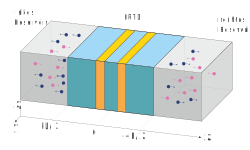
\includegraphics[width=0.7\textwidth]{files/RTD_reservoire.pdf}
  \caption{Veranschaulichung des Modells einer in einen elektrischen Schaltkreis integrierten \ac{rtd}. In den Reservoiren werden Elektronen absorbiert und emittiert. Der in rot angedeutete \emph{Inflow} wird als Randbedingung gesetzt, während der \emph{Outflow} (blau) sich durch die Transportcharakteristik der Bewegungsgleichung ergeben muss.}
  \label{fig:modell}
\end{figure}
Damit ist klar, dass Randbedingungen für Inflow-Teilchen mit positiver Geschwindigkeit am linken Rand und solche mit negativer Geschwindigkeit am rechten Rand der Domäne gesetzt sind, während für Outflow-Teilchen keine Randbedingung vorgegeben ist. Teilchen müssen also nach ihrer Geschwindigkeit unterschieden werden können.
Es ist daher ein natürliches Vorgehen, nach einer Wahrscheinlichkeitsverteilung im Phasenraum zu fragen, siehe Kapitel \ref{sec:wigner}.
Positive und negative Geschwindigkeiten lassen sich einfach durch das Vorzeichen von $k$ unterscheiden, sodass sich die Randbedingungen konkretisieren lassen:
\begin{equation}
  \begin{aligned}
    f_{(1)}(k,-L/2)|_{k>0} &= f_l({k}) \\
    f_{(1)}(k,+L/2)|_{k<0} &= f_r({k})
  \end{aligned}
  \label{eq:rb1}
\end{equation}
Die Gleichgewichts-Verteilung der Reservoire $f_{l,r}(k)$ folgt aus der Fermi-Dirac-Statistik durch Integration über die zwei freien Richtungen $k_x$ und $k_y$. Die Berechnung findet sich im Anhang \ref{sec:A_2} wieder. Es folgt
\begin{align}
  f_{l,r} (k) = \frac{m}{\pi\hbar^2\beta} \ln(1+\exp(\beta(\frac{- k^2\hbar^2}{2m} + \mu))) \; .
  \label{eq:rb2}
\end{align}
und wegen Gleichung \eqref{eq:fourier_wigner_invers} für die reduzierte Dichtematrix
\begin{equation}
  \begin{aligned}
    \rho_{(1)}(x=\pm L/2, y, t) &= \int \frac{\diff k}{2\pi} e^{iky} f(k,\pm L/2) \\
                                &= \int \frac{\diff k}{2\pi} \cos(ky) f_{\nicefrac{r}{l}} (k) \; .
  \end{aligned}
  \label{eq:rb4}
\end{equation}
Das chemische Potential $\mu$ ergibt sich dabei aus der Forderung nach Ladungsträgerneutralität im thermischen Gleichgewicht. Die Herleitung ist im Anhang \ref{sec:A_3} gezeigt.\\
Für die Ausström-Bereiche (auch \emph{Outflow} genannt) $\{ k<0, x=-L/2 \}$ und $\{ k>0, x=+L/2 \}$ trifft \eqref{eq:rb1} keine Aussage, sodass jede numerische Methode zwangsläufig ein Upwind-Schema bezüglich der $r$-Diskretisierung verwenden muss. Hierin bestätigt sich auch der Charakter der zugrundeliegenden Differentialgleichung \eqref{eq:wigner}: es wird der Transport von Elektronen beschrieben.

Eine mögliche Wahl der Randbedingungen bezüglich der Relativkoordinate für die \ac{lvn} sind Dirichlet-Randbedingungen:
\begin{equation}
  \begin{aligned}
    \rho_{(1)}(x, y=\pm L_y/2, t) = 0
  \end{aligned}
  \label{eq:rb3}
\end{equation}
Numerische Resultate zeigen für diese Wahl jedoch mitunter unphysikalische Interferenzmuster, da es an den Rändern zu Reflexion kommt \cite{lukas1}. Ein Vorschlag ist daher, eine absorbierende Schicht (\emph{\ac{cap}}\index{complex absorbing potential}) der Dicke $\delta$ einzuführen. Dabei wird der Driftterm $B(x,y,t)$ aus Gleichung \eqref{eq:lvn} um einen komplexen Teil der Größe $W_0<0$ erweitert:
\begin{equation}
  \begin{aligned}
    B(x,y,t) = \frac{V\left(x+\frac{y}{2},t\right) - V^*\left(x-\frac{y}{2},t\right)}{V_0} + iW(y) \qquad \text{mit} \\
  W(y)=
  \begin{cases}
  W_0 \left(y-\frac{L_y}{2}+\delta \right)^2, & \text{falls}~\frac{L_y}{2}-\delta \le y \le \frac{L_y}{2}\\
  W_0 \left(y+\frac{L_y}{2}-\delta \right)^2, & \text{falls}~-\frac{L_y}{2} \le y \le -\frac{L_y}{2}+\delta\\
  0 & \text{sonst}
  \end{cases}
  \end{aligned}
  \label{eq:cap}
\end{equation}

Die bislang beschriebenen Randbedingungen (Gleichung \eqref{eq:rb1} bzw. \eqref{eq:rb2}) sind als konventionelle oder auch U-Randbedingungen bekannt \cite{failure}. Daneben gibt es weitere Ansätze, wie absorbierende Randbedingungen \cite{arnold1994absorbing, lukas2, lukas1} und Struktur-adaptive Randbedingungen \cite{jiang2014device}. Der Grund für die Suche nach anderen Randbedingungen liegt zum Einen in der Annahme, dass an den Kontakten keinerlei Rückkopplung der Struktur  für die Elektronen zu spüren ist. Im Grenzfall einer unendlich ausgedehnten Struktur ist dies sicherlich gut begründet. Numerische Berechnungen erfordern jedoch stets ein endliches Rechengebiet. Ferner sind physikalische Strukturen immer endlich und durch echte Volumina gekennzeichnet. Korrekte Randbedingungen setzen demnach das Wissen über den Zustand des Systems voraus \cite{ringhofer}.
Kriman et al. \cite{kriman1987scattering} haben gezeigt, dass Quanteneffekte über einige thermische Wellenlängen abklingen. In \cite{ringhofer} wird für eine typische GaAs Struktur bei $\SI{300}{\kelvin}$ eine Abklinglänge von ca. $\SI{100}{\nano\meter}$ angegeben.

Zweitens ist nicht geklärt, wie Randbedingungen bezüglich der Relativkoordinate in der Ortsraumformulierung zu setzen sind. Die meisten Arbeiten beschäftigen sich mit der Wigner-Gleichung \eqref{eq:wigner}. Im Gegensatz zur \ac{lvn} taucht keine zweite Ableitung auf, sodass bezüglich der $k$-Richtung keine Randbedingungen benötigt werden \cite{frensley2}.
Es ist also insbesondere die Thematik der Randbedingungen, worin sich die beiden Formalismen unterscheiden, wodurch also die Äquivalenz von Wigner- und Schrödingerformalismus aufgehoben wird \cite{li2014stationary}.

Die Arbeit von Rosati et al. \cite{failure} weist darauf hin, dass die von Frensley eingeführten Inflow-Randbedingungen zwar semiklassisch zulässig sind, jedoch ihre Verwendung für quantenmechanische Probleme im Allgemeinen nicht gerechtfertigt ist. Dies lässt sich auf die Tatsache zurückführen, dass die semiklassische Boltzmann-Gleichung lokal in $k$ ist, während das quantenmechanische Pendant -- die Wigner-Gleichung -- nicht-lokal in $k$ ist, denn durch die Faltung in Gleichung \eqref{eq:wigner} entsteht eine Kopplung zwischen $k$ und allen anderen $k$-Punkten.
Die Autoren  des Artikels gehen unter Bezug auf den Wigner-Formalismus zwei grundlegenden Fragen nach.
\begin{enumerate}[label=(\roman*)]
  \item Ist die Lösung der Differentialgleichung mit den gegebenen Randbedingungen physikalisch akzeptabel? Für die Dichtematrix bedeutet dies insbesondere, dass sie zu positiver Ladungsträgerdichte führen muss.
  \item Ist die Lösung eindeutig?
\end{enumerate}
Während die semiklassische Boltzmann-Gleichung aufgrund ihres lokalen Charakters eine eindeutige Lösung besitzt, ist dies für die Wigner-Gleichung nicht der Fall. Abbildung \ref{fig:nonuniqueness} zeigt exemplarisch verschiedene stationäre Lösungen für den analytisch lösbaren Fall eines $\delta$-Potentials.
\begin{figure}
  \centering
  \includegraphics[width=0.7\textwidth]{files/nonuniqueness.png}
  \caption{Nicht-Eindeutigkeit der Wigner-Gleichung für den Fall eines $\delta$-Potentials, \cite{failure}.}
  \label{fig:nonuniqueness}
\end{figure}
Die Lösungen ergeben sich dabei aus einer Linearkombination von generischen Vorwärts- und Rückwärts-Streuzuständen, resultierend aus der Zeitumkehr-Symmetrie der stationären Gleichung. Letztere äußert sich auch in der energetischen Zweifach-Entartung der Streuzustände. Eine kurze Rechnung zeigt nämlich, dass wegen der Antisymmetrie des Wignerpotentials sowie der Gruppengeschwindigkeit $v(k) = \hbar k/m$ bezüglich $k$ für jede Lösung $f_{(1)}(k,r)$ auch ${g_{(1)}(k,r) = f_{(1)}(-k,r)}$ Lösung der stationären Wigner-Gleichung ist. Die Randbedingungen geben zwar eine eindeutige Überlagerung, also einen eindeutigen Satz von Koeffizienten $\{a(k)\}$  aller Vorwärts-Streuzustände vor. Da jedoch die Rückwärts-Streuzustände im Allgemeinen linear unabhängig von den Vorwärts-Streuzuständen sind, ist mit denselben Randbedingungen ein doppelt so großer Satz $\{a(k),b(k)\}$ von Koeffizienten zu finden. Das zuvor eindeutige Problem ist in diesem Fall nicht mehr eindeutig lösbar. In der Abbildung sind drei verschiedene Verhältnisse $c=b(k)/a(k)$ zu sehen, darunter auch eine unphysikalische Lösung mit negativer Teilchendichte. Für ausschließlich lokalisierte Zustände, wie sie bei parabolischen oder Quantentopf-Potentialen (mit unendlich großen Barrieren) entstehen, lässt sich jedoch nicht zwischen Vorwärts- und Rückwärts-Streuzuständen unterscheiden sodass eine eindeutige Lösung der Wigner-Gleichung zu erwarten ist \cite{failure}.

Es ist anzumerken, dass dieselbe Argumentation  im allgemeinen Fall der transienten Wigner-Gleichung nicht funktioniert. Dieses Anfangsproblem ist hingegen eindeutig lösbar, wie die Ausarbeitung in \cite{dimov2015boundary} zeigt. Es ist daher zu schlussfolgern, dass die Vorgabe einer Anfangsbedingung zu einer spezifischen Lösung aus der unendlichen Menge möglicher stationärer Lösungen führt, und somit die Anfangsbedingung das entscheidende Kriterium für eine physikalisch akzeptable Problemstellung darstellt. Die Wigner-Gleichung erhält in Bezug auf den Anfangszustand darüber hinaus sogar die Eigenschaft (i) \cite{dimov2015boundary}.

Die vorangegangenen Gedanken lassen sich auf die \ac{lvn} übertragen. Insbesondere die Inversionssymmetrie der stationären Lösung soll im Folgenden gezeigt werden. Es sei $u(x,y)$ Lösung der stationären \ac{lvn} \eqref{eq:lvn_stat}. Dann ist wegen $B(x,y)=-B(x,-y)$ auch $v(x,y)\equiv u(x,-y)$ Lösung, denn
\begin{align*}
  & &-\partial_x \partial_{\xi} u(x,{\xi}) &= - B_{\infty}(x,{\xi})u(x,{\xi}) \\
  &\Leftrightarrow &\partial_x \partial_y u(x,-y) &= - B_{\infty}(x,-y)u(x,-y) \\
  & & &=  B_{\infty}(x,y)u(x,-y) \\
  &\Leftrightarrow &\partial_x \partial_y v(x,y) &=  B_{\infty}(x,y)v(x,y) \; .
\end{align*}

Abschließend ist zu sagen, dass die gesamte Thematik der Randbedingungen Gegenstand aktueller Forschung ist und die hier gezeigten Aspekte nur einen kleinen Bruchteil der Komplexität darstellen. So verkompliziert sich die gesamte Fragestellung beispielsweise dramatisch, wenn die Mean-Field-Näherung fallengelassen wird und auch nicht-kohärente Effekte berücksichtigt werden. Eine gute Übersicht bieten die Arbeiten von Rossi \cite{buchRossi} und Frensley \cite{frensley}. Für die konkrete numerische Implementierung wird auf die vergleichsweise simplen Resultate \eqref{eq:rb1}, \eqref{eq:rb3} sowie für Versuchszwecke Gleichung \eqref{eq:cap} zurückgegriffen.

\section{Weitere Verfahren}\label{sec:weitere_verfahren}
Neben dem hier verwendeten Dichtematrix- bzw. Wigner-Formalismus gibt es einige weitere Möglichkeiten, die stationäre Lösung sowie die Zeitentwicklung für verschiedene Fälle (Gleichgewicht, Nahe-Gleichgewicht und Fern-vom-Gleichgewicht) zu berechnen. Der Artikel \cite{frensley3} bietet einen guten Überblick über die wichtigsten Verfahren. Eine vollständige Theorie gelingt demnach lediglich mit dem \emph{\ac{negf} approach}\index{nonequilibrium Green's function}, welcher auf den Keldysh-Formalismus zurückzuführen ist. Die Grundidee dabei ist eine diagrammatische Störungstheorie, welche sowohl Vorwärts- als auch Rückwärts-Konturen mit Hilfe von vier Greens-Funktionen berücksichtigt. Die konkrete, vollständige Berechnung mit Hilfe der \ac{negf} gestaltet sich anscheinend schwierig. Die Veröffentlichungen konzentrieren sich zumeist auf Hybridverfahren (z.B. \cite{memory2, negf-dft}) oder Spezialfälle wie dem stationären Fall \cite{negf_datta}.
An dieser Stelle soll lediglich festgehalten werden, dass in einer hierarchischen Betrachtungsweise der Dichtematrix-Formalismus weniger Information enthält, denn die Dichtematrix folgt aus einer Integration
\begin{equation*}
  \rho(x,y,t) = \int \frac{\diff E}{2\pi}G^{<}(x,y;E,t) \; .
\end{equation*}
Deshalb ist die \ac{lvn} lediglich dazu in der Lage, ein Markov-Verhalten zu beschreiben, wo also externe Wechselwirkung ausschließlich instantan in der Zeit erfolgt \cite{frensley3}. Als Beispiel für das Versagen des Dichtematrix-Formalismus wird die resonante Absorption oder Emission eines Phonons genannt, für die die Schwingungsperiode des Phonons die Mindestdauer der Wechselwirkung vorgibt. Ein Verfahren, dessen Verteilungsfunktion nicht von allen drei Variablen -- Ort, Impuls und Geschwindigkeit -- abhängt, wird für die entsprechend fehlende Variable eine Erhaltungsgleichung nicht berücksichtigen \cite{frensley3}. Im Falle der \ac{lvn} ist dies die Energieerhaltung, was jedoch mit der Modellierung des Systems vereinbar und sogar notwendig ist, siehe Kapitel \ref{sec:modellierung}. Es gibt Ansätze, diesem Umstand mit Hilfe eines "Gedächtnis-Terms" beizukommen \cite{memory1, memory2}.

Ein Verfahren, welches den Spezialfall des stationären Problems im Gleichgewichtsfall beschreiben kann, wird im folgenden Kapitel \ref{sec:TFmethod} erläutert werden, denn es dient für die numerischen Tests in Kapitel \ref{sec:rates} als Referenz. Eine numerische Beschreibung, welche nicht analytisch, sondern mit der Finiten Elemente Methode die Schrödingergleichung löst und dabei die Offenheit des Systems berücksichtigt, wurde von Lent und Kirkner \cite{qtbm} erarbeitet und ist als \ac{qtbm} bekannt.

\subsection{Transfermatrix Methode}\index{Transfermatrix Method}
\label{sec:TFmethod}
Die Berechnung von reinen Zuständen ist unter Annahme der Stetigkeit von $\Psi(x)$ und $\Psi'(x)$ für den Gleichgewichtsfall anhand Gleichung \eqref{eq:schroedinger} analytisch möglich. Dazu wird als Lösung eine Linearkombination von rechts- und linkslaufender ebener Welle angenommen:
\begin{equation*}
  \begin{aligned}
    \Psi_k(z)=
    \begin{cases}
    a_{l,1}e^{ikz} + a_{l,2}e^{-ikz}              & z\in[-L/2,z_1] \\
    c_{l,1}e^{i\kappa z} + c_{l,2}e^{-i\kappa z}  & z\in[z_1, z_2] \\
    a_{m,1}e^{ikz} + a_{m,2}e^{-ikz}              & z\in[z_2,z_3] \\
    c_{r,1}e^{i\kappa z} + c_{r,2}e^{-i\kappa z}  & z\in[z_3, z_4] \\
    a_{l,1}e^{ikz} + a_{l,2}e^{-ikz}              & z\in[z_4, +L/2] \\
    \end{cases}
  \end{aligned}
\end{equation*}
Hierbei ist $k=\sqrt{2mE/\hbar^2}$ und $\kappa=\sqrt{2m(V_0-E)/\hbar^2}$.
Für das konkrete Problem einer \ac{rtd} zeigt Abbildung \ref{fig:tf1} die Zuordnung der Koeffizienten und Koordinaten.
\begin{figure}
  \centering
  \includegraphics[width=0.7\textwidth]{files/TF_variables.pdf}
  \caption{Koeffizienten für hin- und rücklaufende Wellen mit angedeutetem Potentialverlauf der \ac{rtd}.}
  \label{fig:tf1}
\end{figure}
Mit Hilfe der erwähnten Stetigkeitsbedingung lassen sich acht der zehn Koeffizienten eliminieren, sodass sich mit $\vec{a}\equiv(a_1, a_2)^T$ letztlich
\begin{equation*}
  \vec{a_r} = \underline{\underline{S}} \vec{a_l}
\end{equation*}
schreiben lässt. Dabei hängt die Transfermatrix $\underline{\underline{S}}$ von der Energie $E(k)$ ab und ihre Existenz ist für $k\neq 0$ sichergestellt.
\todo{Der Fall $k=0$  } Die verbliebenen zwei Freiheitsgrade repräsentieren die Notwendigkeit der Randbedingungen. Nun ist es wichtig, die Anforderungen aus Kapitel \ref{sec:modellierung} korrekt zu berücksichtigen. Eingespeiste Elektronen kommen entweder von links, oder von rechts. Sie werden dabei vollständig dekorreliert angesehen, daher muss ${a_{r,2}=1-a_{l,1}}$ und ${a_{l,1}\in\{0,1\}}$ gelten.

Um nun aus der Energie-abhängigen Wellenfunktion die Dichtematrix zu errechnen, wird Gleichung \eqref{eq:dichteoperator} verwendet:
\begin{equation*}
  \rho(x,y) = \sum_k \omega_k \underbrace{\bra{x}\ket{k}}_{\equiv\Psi_k(x)}\bra{k}\ket{y}
\end{equation*}
Der Übergang vom Ein- zum $N$-Teilchen System gelingt, indem nun die Normierung $\sum_k \omega_k = 1$ fallen gelassen und
\begin{equation*}
  \sum_k \omega_k  \Psi_k(x) \Psi_k^{\dagger}(y) \rightarrow \int \diff k \frac{m}{\pi\hbar^2\beta} \ln(1+\exp(\beta(\frac{- k^2\hbar^2}{2m} + \mu))) \Psi_k(x) \Psi_k^{\dagger}(y)
\end{equation*}
angesetzt wird, vergleiche hierzu auch die Überlegung im Anhang \ref{sec:A_2}. Dazu wird die Wellenfunktion gemäß den obigen Überlegungen als gleichgewichtete Summe von linksseitig (${a_{l,1}=1}$) und rechtsseitig (${a_{r,2}=1}$) eingespeistem Elektron zu
\begin{equation*}
  \Psi_k(x) = \frac{1}{\sqrt{2}}(\Psi_k^r(x) + \Psi_k^l(x))
\end{equation*}
gewählt. Das vorgestellte Verfahren ist als \ac{tf} bekannt.



% \section{Herleitung der Liouville-von-Neumann Gleichung}
% Die Liouville-von-Neumann Gleichung erhalten wir aus der von-Neumann-Gleichung wie folgt.
% \begin{align}
%   \td{\hat{\rho}}{t} &= \frac{i}{\hbar}\left[\hat{\rho} , H\right] \\
%   \underbrace{\bra{x} \td{\hat{\rho}}{t} \ket{y}}_{= \partial_t \rho(x,y,t)} &= \bra{x}\ket{\frac{i}{\hbar}\left[\hat{\rho} , H\right]y} \\
%    &= \frac{i}{\hbar} \sum_{\alpha} p_{\alpha} ( \underbrace{\bra{x}\ket{\Psi_{\alpha}}}_{\equiv \Psi_{\alpha}(x)}\bra{\Psi_{\alpha}}\ket{Hy} - \bra{x}\ket{H\Psi_{\alpha}}\underbrace{\bra{\Psi_{\alpha}}\ket{y}}_{\equiv \Psi_{\alpha}^*(y)} )
% \end{align}
% Mit dem Hamiltonoperator für ein einzelnes Teilchen in einer Dimension in Ortsdarstellung
% \begin{align}
%   \left[ -\frac{\hbar^2}{2m}\frac{\partial^2}{\partial x^2} + V(x,t) \right] \Psi(x,t) = \bra{x}\ket{H\Psi} \equiv \mathcal{L}(x,t)\Psi(x,t)
%   \label{eq:Liouville-Operator}
% \end{align}
% folgt mit $H^{\dagger} = H$ und temporärer Unterdrückung der Zeitabhängigkeit
% \begin{align}
%   \partial_t \rho(x,y,t) &= \frac{i}{\hbar} \sum_{\alpha} p_{\alpha} \left( \Psi_{\alpha}(x)\mathcal{L}^*(y)\Psi_{\alpha}^*(y) - \mathcal{L}(x)\Psi_{\alpha}(x)\Psi_{\alpha}^*(y) \right) \\
%   &= \frac{i}{\hbar}  (\mathcal{L}^*(y) - \mathcal{L}(x)) \sum_{\alpha} p_{\alpha} \left( \Psi(x)\Psi^*(y) \right) \\
%   &= \frac{i}{\hbar}  (\mathcal{L}^*(y) - \mathcal{L}(x)) \bra{x}\left(\sum_{\alpha} p_{\alpha}  \ket{\Psi_{\alpha}}\bra{\Psi_{\alpha}} \right)\ket{y} \\
%   &= \frac{i}{\hbar}  (\mathcal{L}^*(y) - \mathcal{L}(x))\rho(x,y)
% \end{align}


% frensley3 zu QTBM (S.11)
% This requires that appropriate boundary conditions be formulatedan dap pliedt o
% (35). Lent and Kirkner [18] have demonstrated how to do this in the context of a finite-element electron
% waveguide calculation, andthe ir approach is calledthe Quantum Transmitting Boundary Method (QTBM).
% In the continuous case, one derives the QTBM conditions by evaluating ψ andit s derivative ψ at xl and
% xr using (30). One then solves for the incident amplitudes al and ar in terms of ψ and ψ, and imposes
% the resulting expressions upon Schr¨odinger’s equation as inhomogeneous boundary conditions. Conditions
% of this type, in which a linear combination of the function and its derivative are specified, are known as
% Robbins conditions.This requires that appropriate boundary conditions be formulatedan dap pliedt o
% (35). Lent and Kirkner [18] have demonstrated how to do this in the context of a finite-element electron
% waveguide calculation, andthe ir approach is calledthe Quantum Transmitting Boundary Method (QTBM).
% In the continuous case, one derives the QTBM conditions by evaluating ψ andit s derivative ψ at xl and
% xr using (30). One then solves for the incident amplitudes al and ar in terms of ψ and ψ, and imposes
% the resulting expressions upon Schr¨odinger’s equation as inhomogeneous boundary conditions. Conditions
% of this type, in which a linear combination of the function and its derivative are specified, are known as
% Robbins conditions.

% \chapter{Ergebnisse der Arbeit}

\section{Transfer Function Methode}
\label{sec:TFmethod}

% \input{content/04_zusammenfassung.tex}
%
% \appendix
% % Hier beginnt der Anhang, nummeriert in lateinischen Buchstaben
% % % \chapter{Berechnete Grundenergien der isotropen Spinleiter}
% \label{anh:tabellen}
% Im Folgenden werden die Ergebnisse aus Kapitel \ref{sec:grundzustand} ergänzt um die entsprechenden Werte für \(J_\parallel\in\{0,2\;\;0,4\;\;0,6\;\;0,8\}\). Dies dient dem vollständigen Vergleich gegenüber der Berechnung aus \cite{4}.
% \input{files/Tabelle_Jperp_0.2_texformat.tex}
% \input{files/Tabelle_Jperp_0.4_texformat.tex}
% \input{files/Tabelle_Jperp_0.6_texformat.tex}
% \input{files/Tabelle_Jperp_0.8_texformat.tex}

\chapter{Anhang}
\section{Ortsbasis}
\label{sec:A_1}
Für ein einzelnes Teilchen beispielsweise ist letztere die Menge der Eigenvektoren des Orstoperators
\begin{equation*}
  X:D_X \rightarrow L^2(\mathbb{R}^3;\mathbb{C}) \, : \, \Psi \mapsto x\Psi
\end{equation*}
zu den (i.A. komplexen) Eigenwerten $x$. Hierbei ist $D_X$ die Domäne
\begin{equation*}
  D_X = \{\Psi \in L^2(\mathbb{R}^3) \, | \, x\Psi \in L^2(\mathbb{R}^3)
\end{equation*}
des selbstadjungierten Operators $X$. Mit anderen Worten ist für eine Teilchenzahl $N$ der Zustand $\ket{x}$ derjenige Zustand, für den der Aufenthaltsort jedes Teilchens exakt bekannt (mit $x$ zusammengefasst) und wegen der Unschärferelation der Impuls vollständig unbekannt ist.
%Hierbei ist $S(\mathbb{R}^3)*$ der Raum der komplexwertigen temperierten Distributionen.
% S^* ist Dualraum des "Schwartz-Raums", welcher wiederum in allen Sobolew-Räumen enthalten ist. (Wiki) Der Raum der Testfunktionen lässt sich stetig in den Schwartz-Raum einbetten und liegt in diesem dicht.
die $\ket{x}$ stellen als Kontinuum eine uneigentliche Basis dar. Für die Spurbildung ist folglich ein Integral über $D_X$ auszuführen, statt einer Summation.

\section{Integration der Fermi-Dirac-Statistik}
\label{sec:A_2}
Im Folgenden wird die Teilchendichte (Teilchenzahl pro Fläche) für bezüglich $x$- und $y$- Richtung freie Elektronen im großkanonischen Ensemble mit chemischem Potential $\mu$ hergeleitet. Dabei ist die Fermi-Dirac-Statistik gemäß Gleichung \eqref{eq:wigner_n} über alle möglichen Impulse $\vec{k}=(k_x,k_y,k_z)$ zu integrieren. Allerdings ist die Dispersionsrelation bzgl. $k_z$ nicht bekannt, weshalb diese Variable zunächst als Freiheitsgrad beibehalten wird.
\begin{align*}
  \frac{\expval{N}}{A_{\perp}} &= 2\frac{1}{A_{\perp}}\sum_{\vb{k}}\frac{1}{1+\exp(\beta(\epsilon(\vb{k}) - \mu))} \\
    &= 2\frac{1}{A_{\perp}}  \frac{A_{\perp}}{(2\pi)^2} \sum_{k_z}\int_{-\infty}^{\infty} \diff k_y \int_{-\infty}^{\infty} \diff k_x \frac{1}{1+\exp(\beta(k_x^2 + k_y^2 + k_z^2)\frac{\hbar^2}{2m} - \mu)} \\
    &= \frac{2}{(2\pi)^2} \sum_{k_z} \int_0^{2\pi} \diff \varphi \int_0^{\infty} \diff k_{\perp} k_{\perp} \frac{1}{1+\exp(\beta(k_{\perp}^2 + k_z^2)\frac{\hbar^2}{2m} - \beta \mu)}
\end{align*}
Substitution von $\epsilon = (k^2_{\perp} + k_z^2)\frac{\hbar^2}{2m} - \mu$ und somit $\diff k_\perp = \frac{m}{\hbar^2 k}\diff \epsilon$ sowie der Zusammenhang $\td{}{x}\ln(1+\exp(-\beta x)) = -\beta / (1+\exp(\beta x))$ liefern
\begin{align*}
  \frac{\expval{N}}{A_{\perp}} &= \frac{4\pi}{(2\pi)^2} \frac{m}{\hbar^2} \sum_{k_z} \int_{\epsilon(0)}^{{\epsilon(\infty)}} \diff \epsilon \frac{1}{1+\exp(\beta\epsilon)} \\
    &= \frac{m}{\pi\hbar^2}\left( \frac{-1}{\beta}\right) \sum_{k_z} \left.\ln(1+\exp(-\beta(k_{\perp}^2 + k_z^2)\frac{\hbar^2}{2m} + \beta\mu))\right|_0^{\infty} \\
    &= \sum_{k_z} \frac{m}{\pi\hbar^2\beta} \ln(1+\exp(\beta(\frac{- k_z^2\hbar^2}{2m} + \mu)))
\end{align*}
Für lokal konstantes $\beta$ folgt daher in Übereinstimmung mit \cite{frensley2} die Beschreibung der Reservoire gemäß
\begin{align}
  f_{l,r} (k) = \frac{m}{\pi\hbar^2\beta} \ln(1+\exp(\beta(\frac{- k^2\hbar^2}{2m} + \mu_{l,r}))) \; .
\end{align}

\section{Chemisches Potential }
\label{sec:A_3}
Das chemische Potential der Kontakte ergibt sich aus der Forderung nach Ladungsneutralität unter Kenntnis der Dotierung von Donatoren $N_D$ und Akzeptoren $N_A$. Für $n$-dotiertes GaAs gilt demnach
\begin{equation}
  0 = N_D - p + N_A - n \approx N_D - n(\mu) \equiv f(\mu)
\end{equation}
Die Elektronendichte folgt aus Zustandsdichte und Fermi-Dirac-Verteilung gemäß
\begin{align}
  n(\mu) &= \int\diff E \rho(E) f(E) \\
   &= \int_{E_c}^{\infty}\frac{(2m)^{\nicefrac{3}{2}} }{2\pi^2\hbar^3}\sqrt{E-E_c} \frac{1}{1+e^{\beta(E-E_c-\mu)}}
\end{align}
Die Leitungsbandkantenenergie $E_c$ der GaAs-Schicht wird zu 0 gewählt. Das chemische Potential wird aus der Nullstellensuche $f(\mu)=0$ mit einem Newton-Raphson-Verfahren ermittelt. Numerisch ergibt sich für den Gleichgewichtsfall  $\mu\approx\SI{0.04617}{\electronvolt}$.

\section{Hartree-Potential}\index{Hartree-Potential}\label{sec:A_4}
Das Hartree-Potential ist mit der Elektronendichte $n(\vb{x})$ durch die \emph{Poisson-Gleichung}\index{Poisson-Gleichung} \cite{frensley}
\begin{align}
  -\div \epsilon(\vb{x}) \grad u(\vb{x}) = e^2 (n(\vb{x}) - N_D(\vb{x})) \; ,
  \label{eq:poisson_3d}
\end{align}
verknüpft, wobei $N_D(\vb{x})$ die ortsabhängige Dichte der Donatoren in der Heterostuktur und $\epsilon(\vb{x})$ die Permittivität bezeichnet. Akzeptoren und Löcher werden aufgrund der Dotierung $N_D \gg N_A$ vernachlässigt. Ferner ist aufgrund der eindimensionalen Problemstellung anzunehmen, dass $u(\vb{x}) = u(x)$ und $\epsilon(\vb{x})=\epsilon(x)$ sodass die Poisson-Gleichung eindimensional wird.
\begin{align}
  -\partial_x (\epsilon(x)\partial_x u(x)) = e^2(n(x)-N_D(x))
  \label{eq:poisson}
\end{align}
Die Randbedingungen für $u$ ergeben sich aus der Forderung nach Ladungsneutralität in ausreichend großer Entfernung gemäß \cite{frensley}
\begin{align}
  u|_{\partial\Omega} = \mu(\vb{x})|_{\partial\Omega}-V_s(\vb{x})|_{\partial\Omega}-\frac{1}{\beta}\mathcal{F}_{1/2}^{-1}(N_D/N_C) \; .
  \label{eq:RB_PE}
\end{align}
Hierin ist $\mu(\vb{x})$ das chemische Potential, $\beta=1/(k_BT)$ mit $T=\SI{300}{\kelvin}$, $N_C = 2(m^*/2\pi\hbar^2\beta)^{3/2}$ die "effektive Zustandsdichte" und $\mathcal{F}_{1/2}$ das Fermi-Dirac Integral der Ordnung $1/2$:
\begin{align}
  \mathcal{F}_j(x)=\frac{1}{\Gamma(j+1)}\int_0^{\infty}\frac{t^j}{\exp(t-x)+1}\diff t
\end{align}
Das Potential ergibt sich nach Gleichungen \eqref{eq:poisson} und \eqref{eq:expval_n} aus dem Dichteoperator -- umgekehrt ergibt sich der Dichteoperator nach Gleichung \eqref{eq:lvn} aus dem Potential. Die Beziehung zwischen Potential und Dichte ist nicht-linear. Die gleichzeitige Lösung für Poisson-Gleichung und \ac{lvn} zu finden erfordert daher Iteration. Das Problem wird \emph{selbstkonsistent} gelöst. Dazu wird $\eqref{eq:lvn}$ zunächst mit einem geeigneten \emph{initial guess} $V^{(0)}$ gelöst. Nun wird iteriert und alternierend gelöst, bis Dichte und Potential sich nicht mehr signifikant ändern. Im Fall der transienten Betrachtung entspricht eine Iteration gleichzeitig einem Zeitschritt. Das Verfahren ist als \emph{Gummel (Plug-in) Approach} etabliert und beispielsweise in \cite{gummel} beschrieben. Die folgenden Ausführungen orientieren sich an dieser Literaturquelle.

Numerisch kann Gleichung \eqref{eq:poisson} mit dem Finite-Differenzen Verfahren behandelt werden. Das Rechengebiet $L$ wird diskretisiert gemäß
\begin{align}
  L_N \equiv \{x_i | x_i = i h \,\forall\, i = 0,1,\dots,N\text{ mit }L=Nh\}
\end{align}
Aus der Taylorentwicklung einer Funktion $f:L \rightarrow \mathbb{R}$ folgt für die Ableitungen
\begin{align}
  f'(x_i) &= \frac{f(x_{i+1}) - f(x_{i-1})}{2h} + \mathcal{O}(h^2) \\
  f''(x_i) &= \frac{f(x_{i+1}) - 2f(x_i) + f(x_{i-1})}{h^2} + \mathcal{O}(h^2) \; .
\end{align}
Die Kurzschreibweise $f(x_i)\equiv f_i$ bietet sich an.
Damit lässt sich mit $a_i\equiv (\epsilon_{i+1} - \epsilon_{i-1})/(4\epsilon_i)$ Gleichung \eqref{eq:poisson} umschreiben zu
\begin{align}
  u_{i+1}\cdot(1+a_i) -2 u_i + u_{i-1}\cdot(1-a_i) - \underbrace{e^2h^2\frac{(N_{D,i} - n_i)}{\epsilon_i}}_{\equiv \text{rhs}_i} = 0\; ,
  \label{eq:discretePE}
\end{align}
wobei berücksichtigt werden muss, dass $u_0$ und $u_N$ über die Randbedingungen nach Gleichung \eqref{eq:RB_PE} vorgegeben sind. Somit ist das LGS
\begin{align}
  \left[ \begin{matrix}-2 & 1+a_1 & & & 0\\1-a_2 & \ddots & \ddots & & \\ & \ddots & \ddots & \ddots & \\& & \ddots & \ddots &  1+a_{N-2} \\0 & &  & 1-a_{N-1} & -2  \end{matrix}  \right]
  \left[ \begin{matrix}u_1             \\                          \\ \vdots                       \\                           \\u_{N-1}  \end{matrix}  \right]
  = \left[ \begin{matrix}\text{rhs}_1  \\                          \\ \vdots                       \\                         \\\text{rhs}_{N-1}  \end{matrix}  \right]
   - \left[ \begin{matrix}(1-a_1)u_0     \\0                         \\ \vdots                      \\0                        \\(1+a_{N-1})u_N  \end{matrix}  \right]
\end{align}
zu lösen. Die Frage nach einer "besseren" Vorhersage für $u^{(n+1)}$ und damit einer schnelleren Konvergenz der Iteration führt auf das verallgemeinerte Newton-Raphson-Verfahren.
Die linke Seite von Gleichung \eqref{eq:discretePE} wird als Funktion $P_i(u_1,\dots,u_N)$ definiert, worauf das Newton-Raphson-Verfahren angewandt wird. Ausgehend von einem Startwert $\vb{u}^{(0)}$ ergibt sich das Fixpunktproblem
\begin{align}
  \vb{u}^{(n+1)} = \vb{u}^{(n)} - (\mathrm{D}\vb{P}|_{\vb{u}^{(n)}})^{-1} \vb{P}(\vb{u}^{(n)}) \; ,
  \label{eq:fixpunkt_gummel}
\end{align}
wobei die Vektorschreibweise
\begin{align}
  \vb{f} = \left( f_0,\dots,f_N\right)^T = \left( f(x_0),\dots,f(x_N)\right)^T
\end{align}
eingeführt worden ist und $\mathrm{D}$ der Differentiationsoperator ist, in diesem Fall also die Jacobimatrix von $P$.
\begin{align}
  \left(\mathrm{D}\vb{P}|_{\vb{u}^{(n)}}\right)_{i,j} &= \pd{P_i}{u_j^{(n)}} \\ &\stackrel{\eqref{eq:discretePE}}{=}
  (1+a_i)\delta_{i+1,j} - 2 \delta_{i,j} + (1-a_i)\delta_{i-1,j} + \frac{e^2h^2}{\epsilon_i}\pd{n_i^{(n)}}{u_j^{(n)}}
\end{align}
An dieser Stelle ist anzumerken, dass nun auch die Dichte $n$ einen Iterationsindex $(n)$ bekommen hat. Dies ist auf die eingangs beschriebene alternierende Iteration zurückzuführen, in welcher abwechselnd $n^{(n)}$ und $u^{(n)}$ in einem einzigen Iterationsschritt $(n)$ berechnet werden. Ferner ist die Ableitung $\pd{n_i^{(n)}}{u_j^{(n)}}$ zunächst nicht bekannt.
Es ist überhaupt eine Abweichung $\pd{n_i^{(n)}}{u_j^{(n)}} \neq 0$, die den Unterschied zwischen Newton-Iteration und direktem Lösen bewirkt. Im Allgemeinen liegt keine exakte Form dieser Ableitung vor, da hierzu ja gerade die \ac{lvn} zu lösen ist. Es lässt sich jedoch eine Abschätzung vornehmen, welche schnell und kostengünstig ist, sodass das Newton-Verfahren einen echten Vorteil gegenüber dem direkten Iterieren hat. Dazu dient die Maxwell-Boltzmann-Statistik
\begin{align}
  n(u) = N_0\exp\left(\frac{u-u_0}{k_B T}\right)
  \label{eq:maxwell_boltzmann}
\end{align}
als klassisches Gleichgewichts-Resultat. Dies ist wohlgemerkt eine Annahme und es lassen sich ebenso andere Annehmen, z.B. eine Fermi-Dirac-Statistik, wählen. Jedoch zeigt sich in der Praxis, dass diese Wahl zuverlässig zu einer Konvergenz des Verfahrens führt. Falls nicht stationär, sondern transient gelöst werden soll, sollte jedoch das Newton-Verfahren nicht verwendet werden, da ein Iterationsschritt hier einem Zeitschritt entspricht und die Annahme \eqref{eq:maxwell_boltzmann} heuristischer Natur ist. Somit würde physikalisches Verhalten implizit aufgeprägt werden, statt dass dieses durch die vorhandenen zwei Gleichungen beschrieben wird.

Für den stationären Fall folgt aus Annahme \eqref{eq:maxwell_boltzmann} für das diskretisierte System
\begin{align}
  \pd{n_i}{u_j} = \frac{n_i}{k_B T}\delta_{i,j} \; .
\end{align}
Statt die Jacobi-Matrix invertieren zu müssen, ist es geschickter, Gleichung \eqref{eq:fixpunkt_gummel} umzuschreiben:
\begin{align}
  \mathrm{D}\vb{P}|_{\vb{u}^{(n)}}(\vb{u}^{(n+1)} - \vb{u}^{(n)}) = -  \vb{P}(\vb{u^{(n)}})
\end{align}
Explizit ausgeschrieben gilt
\begin{align}
  \left(\mathrm{D}\vb{P}|_{\vb{u}^{(n)}}\right)_{i,j} &=
    (1+a_i)\delta_{i+1,j} + ( \frac{e^2h^2}{\epsilon_i}\frac{n_i}{k_B T} - 2) \delta_{i,j} + (1-a_i)\delta_{i-1,j} \\
  \left( \vb{P}(\vb{u^{(n)}}) \right)_{i} &=
   u_{i+1}^{(n)}\cdot(1+a_i) -2 u_i^{(n)} + u_{i-1}^{(n)}\cdot(1-a_i) - e^2h^2\frac{(N_{D,i} - n_i^{(n)})}{\epsilon_i}
\end{align}
mit $i,j = 1,\dots,N-1$. Lösen des LGS für $(\vb{u}^{(n+1)} - \vb{u}^{(n)})$ führt zu
\begin{align}
  \vb{u}^{(n+1)} = (\vb{u}^{(n+1)} - \vb{u}^{(n)}) + \vb{u}^{(n)} \; .
\end{align}

\section{Herleitung der Driftmatrix}\index{Driftmatrix}\label{sec:A_5}
Im Folgenden soll der Ausdruck \eqref{eq:G_GL} ausgehend von der Definition \ref{def:matrizen} der Driftmatrix
\begin{equation*}
  (\drift^{k,jm})_{pq} = \int_{D^k} G_{jm}(x) \ell_p^k(x) \ell_q^k(x) \diff x \qquad \forall j,m=1\dots K_y % v_{\mathcal{T},p}^{k,m} wird dadran multipliziert
\end{equation*}
hergeleitet werden. Dazu wird zunächst Gleichung \eqref{eq:ellPsi} angewandt, also
\begin{equation*}
  \ell_i(x) = \sum_{n=1}^{N_p} (\van^T)^{-1}_{in}\Phi_n(x) \; .
\end{equation*}
Es folgt
\begin{align*}
    (\drift^{k,jm})_{pq} &= \sum_{r,s=1}^{N_p}\int_{D^k} G_{jm}(x) (\van^T)^{-1}_{pr}\Phi_r(x) (\van^T)^{-1}_{qs}\Phi_s(x) \\
     &= \sum_{r,s=1}^{N_p} (\van^T)^{-1}_{pr} (\van^T)^{-1}_{qs}  \int_{D^k} G_{jm}(x) \Phi_r(x) \Phi_s(x) \; .
\end{align*}
Das Integral wird durch die Jacobideterminante $J^k=h^k/2$ auf das Referenzelement $[-1,1]$ überführt und mit Hilfe der Gauß-Lobatto Quadratur mit Knotenpunkten $\xi_i$, Gewichten $w_i$ und Ordnung $N_{GL}$ approximiert:
\begin{align*}
    (\drift^{k,jm})_{pq} &\approx \sum_{r,s=1}^{N_p} (\van^T)^{-1}_{pr} (\van^T)^{-1}_{qs}  \sum_{a=1}^{N_{GL}} G_{jm}(x(\xi_a)) \Phi_r(\xi_a) \Phi_s(\xi_a) w_a J^k\; .
\end{align*}
Mit der Definition der Vandermondematrix $\van_{ij}=\Phi_j(\xi_i)$ aus Gleichung \eqref{eq:vandermonde} lässt sich eine zweite Vandermondematrix $\tilde{\van}$ der Größe $N_{GL}\times N_p$ einführen, sodass
\begin{align*}
  (\drift^{k,jm})_{pq} &= \sum_{r,s=1}^{N_p}\sum_{a=1}^{N_{GL}} (\van^T)^{-1}_{pr} (\van^T)^{-1}_{qs}   G_{jm}(x(\xi_a)) \tilde{\van}_{ar} \tilde{\van}_{as} w_a J^k \\
  &= \sum_{r,s=1}^{N_p}\sum_{a=1}^{N_{GL}} (\van^T)^{-1}_{pr} (\van^T)^{-1}_{qs}   G_{jm}(x(\xi_a)) \tilde{\van}_{ra}^T \tilde{\van}_{sa}^T w_a J^k \\
  &= \sum_{a=1}^{N_{GL}} ((\van^{-1})^T \tilde{\van}^T)_{pa} ((\van^{-1})^T \tilde{\van}^T)_{qa}   G_{jm}(x(\xi_a))   w_a J^k \\
  &= \sum_{a=1}^{N_{GL}} (\tilde{\van} \van^{-1})_{ap} (\tilde{\van} \van^{-1})_{aq}   G_{jm}(x(\xi_a))   w_a J^k
\end{align*}
folgt. Mit der Definition $W\equiv\tilde{\van}V^{-1}$ ergibt sich das gesuchte Resultat \eqref{eq:G_GL}.

%
% \backmatter
% \printbibliography
%
% \cleardoublepage
% \input{content/eid_versicherung.tex}
\end{document}
